% Format teze zasnovan je na paketu memoir
% http://tug.ctan.org/macros/latex/contrib/memoir/memman.pdf ili
% http://texdoc.net/texmf-dist/doc/latex/memoir/memman.pdf
% 
% Prilikom zadavanja klase memoir, navedenim opcijama se podešava 
% veličina slova (12pt) i jednostrano štampanje (oneside).
% Ove parametre možete menjati samo ako pravite nezvanične verzije
% mastera za privatnu upotrebu (na primer, u b5 varijanti ima smisla 
% smanjiti 
\documentclass[12pt,oneside]{memoir} 

% Paket koji definiše sve specifičnosti master rada Matematičkog fakulteta
\usepackage[latinica]{matfmaster} 
\usepackage{amsthm}

% Podešavanje stila listinga
\usepackage{listings}
\usepackage{xcolor}

\definecolor{codegreen}{rgb}{0,0.6,0}
\definecolor{codegray}{rgb}{0.5,0.5,0.5}
\definecolor{codepurple}{rgb}{0.58,0,0.82}
\definecolor{backcolour}{rgb}{0.95,0.95,0.92}

\lstdefinestyle{mystyle}{
    backgroundcolor=\color{backcolour},   
    commentstyle=\color{codegreen},
    keywordstyle=\color{magenta},
    numberstyle=\tiny\color{codegray},
    stringstyle=\color{codepurple},
    basicstyle=\ttfamily\footnotesize,
    breakatwhitespace=false,         
    breaklines=true,                 
    captionpos=b,                    
    keepspaces=true,                 
    numbers=left,                    
    numbersep=5pt,                  
    showspaces=false,                
    showstringspaces=false,
    showtabs=false,                  
    tabsize=2
}

\lstdefinestyle{terminal}{
    backgroundcolor=\color{backcolour},   
    basicstyle=\ttfamily\footnotesize,
    breakatwhitespace=false,         
    breaklines=true,                 
    captionpos=b,                    
    keepspaces=true,                                                  
    showspaces=false,                
    showstringspaces=false,
    showtabs=false,                  
}

%\lstset{style=mystyle}


\theoremstyle{plain}
\newtheorem{thm}{Teorema}[chapter] % svaki chapter resetuje brojač

\theoremstyle{definition}
\newtheorem{defn}{Definicija} % definicija
\newtheorem{lem}{Lema} % lema
%
% Podrazumevano pismo je ćirilica.
%   Ako koristite pdflatex, a ne xetex, sav latinički tekst na srpskom jeziku
%   treba biti okružen sa \lat{...} ili \begin{latinica}...\end{latinica}.
%
% Opicija [latinica]:
%   ako želite da pišete latiniciom, dodajte opciju "latinica" tj.
%   prethodni paket uključite pomoću: \usepackage[latinica]{matfmaster}.
%   Ako koristite pdflatex, a ne xetex, sav ćirilički tekst treba biti
%   okružen sa \cir{...} ili \begin{cirilica}...\end{cirilica}.
%
% Opcija [biblatex]:
%   ako želite da koristite reference na više jezika i umesto paketa
%   bibtex da koristite BibLaTeX/Biber, dodajte opciju "biblatex" tj.
%   prethodni paket uključite pomoću: \usepackage[biblatex]{matfmaster}
%
% Opcija [b5paper]:
%   ako želite da napravite verziju teze u manjem (b5) formatu, navedite
%   opciju "b5paper", tj. prethodni paket uključite pomoću: 
%   \usepackage[b5paper]{matfmaster}. Tada ima smisla razmisliti o promeni
%   veličine slova (izmenom opcije 12pt na 11pt u \documentclass{memoir}).
%
% Naravno, opcije je moguće kombinovati.
% Npr. \usepackage[b5paper,biblatex]{matfmaster}

% Pomoćni paket koji generiše nasumičan tekst u kojem se javljaju sva slova
% azbuke (nema potrebe koristiti ovo u pravim disertacijama)

% Datoteka sa literaturom u BibTex tj. BibLaTeX/Biber formatu
\bib{literatura}

% Ime kandidata na srpskom jeziku (u odabranom pismu)
\autor{Lazar S. Mladenović}
% Naslov teze na srpskom jeziku (u odabranom pismu)
\naslov{Automatsko ispravljanje grešaka detektovanih pomoću alata Memcheck }
% Godina u kojoj je teza predana komisiji
\godina{2020}
% Ime i afilijacija mentora (u odabranom pismu)
\mentor{dr Milena \textsc{Vujošević Janičić}, vanredni profesor \\ Univerzitet u Beogradu, Matematički fakultet}
% Ime i afilijacija prvog člana komisije (u odabranom pismu)
\komisijaA{dr Miodrag \textsc{Živković}, redovan profesor\\ Univerzitet u Beogradu, Matematički fakultet}
% Ime i afilijacija drugog člana komisije (u odabranom pismu)
\komisijaB{dr Filip \textsc{Marić}, vanredni profesor\\ Univerzitet u Beogradu, Matematički fakultet}
% Ime i afilijacija trećeg člana komisije (opciono)
% \komisijaC{}
% Ime i afilijacija četvrtog člana komisije (opciono)
% \komisijaD{}
% Datum odbrane (odkomentarisati narednu liniju i upisati datum odbrane ako je poznat)
 \datumodbrane{}

% Apstrakt na srpskom jeziku (u odabranom pismu)
\apstr{
Verifikacija softvera zauzima bitno mesto u procesu razvoja softvera. Dinamička verifikacija softvera zasniva se na proveri ispravnosti softvera koja se vrši tokom njegovog izvršavanja. Postoje razni alati i platforme za dinamičku verifikaciju softvera, a jedna značajna platforma je \textit{Valgrind}. Alati njegove distribucije mogu dati profile programa koji mogu pomoći u poboljšanju rada i performansa programa, a takođe mogu i ukazati na greške u okviru programa koje nije lako otkriti. Važan alat platforme \textit{Valgrind} je \textit{Memcheck}. Ovaj alat analizira i ukazuje na greške u radu sa memorijom. Te greške mogu da izazovu pad programa, a uključuju, na primer, korišćenje neinicijalizovane vrednosti i pristup oslobođenoj, odnosno nedozvoljenoj memoriji. Cilj ovog rada je konstrukcija alata koji će koristeći izvešataj koji daje \textit{Valgrind}, odnosno \textit{Memcheck}, otkriti i ispraviti uzroke grešaka u programu. Osnovna ideja za ostvarivanje ovog cilja je da se definišu relevantni šabloni za ispravljanje grešaka i da se implementira automatska analiza izveštaja koji se dobija iz alata \textit{Memcheck} i koja korišćenjem odgovarajućih šablona postiže željenu funkcionalnost. 
}

% Ključne reči na srpskom jeziku (u odabranom pismu)
\kljucnereci{Verifikacija softvera, dinamička analiza, profajliranje, Valgrind, Memcheck}

\begin{document}
% ==============================================================================
% Uvodni deo teze
\frontmatter
% ==============================================================================
% Naslovna strana
\naslovna
% Strana sa podacima o mentoru i članovima komisije
\komisija
% Strana sa posvetom (u odabranom pismu)
\posveta{Familiji}
% Strana sa podacima o disertaciji na srpskom jeziku
\apstrakt
% Sadržaj teze
\tableofcontents*

% ==============================================================================
% Glavni deo teze
\mainmatter
% ==============================================================================

% ------------------------------------------------------------------------------
\chapter{Uvod}
% ------------------------------------------------------------------------------
Razvoj softvera predstavlja složen proces koji obuhvata razne aktivnosti. Nepisano je pravilo da se prilikom pisanja programa može desiti da se provuče neka greška kao npr. neinicijalizacija promenljive, ili neoslobađanje alocirane memorije, koja u tom trenutku možda biva bezazlena. Međutim, kako razvoj programa odmiče, dodatne greške koje ta početna, naizgled bezazlena greška izaziva, bivaju krucijalne i od vitalnog značaja. Na neke od gore pomenutih grešaka, nažalost kompliator ne može da nam ukaže. Ovo nije veliki problem ukoliko su naši programi mali, ali u  kompleksnijim programima, onim koji se sastoje od više hiljada linija koda, greške je teško naći. 

Verifikacija softvera ima za cilj ispravljanje tih grešaka i zauzima bitno mesto u procesu razvoja softvera. Statička verifikacija softvera analizira ispravnost programa bez njegovog izvršavanja, tj.~vrši analizu izvornog koda, dok dinamička verifikacija softvera predstavlja tehniku ispitivanja ispravnosti koda u toku njegovog izvršavanja \cite{02Motivacija}. Binarna analiza obuhvata analizu na nivou mašinskog koda, snimljenog kao objektni k\^od (nepovezan) ili kao izvršni k\^od (povezan) \cite{03DinamickaAnaliza}. Primer platforme koji vrši dinamičku binarnu analizu koda jeste \textit{Valgrind}.  

\textit{Valgrind} je platforma koja pruža brojne alate za debagovanje i profajliranje koji pomažu da se brže i pravilnije otklone greške u programima. Najpopularniji od ovih alata zove se \textit{Memcheck}. Ovaj alat može otkriti mnoge greške u vezi sa memorijom koje su česte u programima C i C++, a koje mogu dovesti do pada ili nepredvidivog ponašanja programa. 

Platforma \textit{Valgrind} sa svim svojim alatima samo ukazuje na greške, kao i na to šta ih je izazvalo. Ispravljanje istih ostaje programeru. Cilj ovog rada jeste da automatizuje ispravljanje grešaka na koje ukazuje alat \textit{Valgrind}, tako što će koristiti precizno definisane šablone za ispravljanje grešaka. U realizaciji te ideje će se primenjivati regularni izrazi kojima će biti opisani izrazi koji mogu da prouzrokuju greške na koje nam ukazuje \textit{Memcheck}.

U glavi 2 platforma \textit{Valgrind} će biti detaljno opisana. Biće pobrojani i obrađeni svi alati \textit{Valgrind}-a. Najveći akcenat će biti na alatu \textit{Memcheck}, dok će o ostalima biti date osnovne relevantne informacije. U glavi 3 biće ukratko reči o procesu kompilacije programa i njenim fazama. Centralno mesto zauzeće teorija o jezicima i regularnim izrazima. U glavi 4 biće predstavljen alat \textit{Koronka}, koji je osnovni doprinos ovog rada: biće opisana arhitektura, algoritam izvršavanja i njegove funkcionalnosti. Takođe, čitaoci će biti bliže upoznati sa načinom upotrebe i rada alata. Na kraju, biće iznet osvrt na ceo rad. Kako tema to afirmiše, a i sam alat je napravljen tako da može da se stalno unapređuje, u smislu uopštavanja postojećih šablona, primene drugih vrsta analiza i alata \textit{Valgrind}-a i sl., biće iznete i ideje i mogućnosti za dalji razvoj ovog projekta.


\chapter{Alat Valgrind}
\textit{Valgrind}\footnote{ Ime \textit{Valgrind} potiče iz nordijske mitologije.} je platforma za pravljenje alata za dinamičku analizu \cite{Valgrind}. Dolazi sa skupom alata, od kojih svaki obavlja neku vrstu debagovanja, profajliranja ili slične zadatke koji pomažu programeru da poboljša program koji razvija. \textit{Valgrind} se može koristiti i kao alat za pravljenje novih alata, bez narušavanja postojeće strukture. 
\textit{Valgrind} distribucija trenutno broji sledeće alate:
\begin{enumerate}
  \item \textit{Memcheck} \cite{ValgrindDOC} --- alat za detekciju memorijskih grešaka.
  \item \textit{Cachegrind}  \cite{Cachegrind} --- profajler keš memorije i skokova. 
  \item \textit{Callgrind} \cite{Callgrind} --- profajler poziva funkcija.
  \item \textit{Helgrind} \cite{Helgrind} --- alat za detekciju grešaka niti.
  \item \textit{DRD} \cite{Drd} --- alat za detekciju grešaka niti. 
  \item \textit{Massif} \cite{Massif} --- profajler korišćenja dinamičke memorije.
  \item \textit{DHAT} \cite{DHAT} --- profajler korišćenja dinamičke memorije. % predstavlja drugu vrstu profajlera hipa koji pomaže u razumevanju problema sa životnim vekom bloka, upotrebom bloka i neefikasnošću rasporeda.
  \item \textit{BBV} \cite{BBV} --- eksperimentalni alat za podršku razvoja novih arhitektura računara. % eksperimentalni alat za generisanje osnovnih vektorskih blokova za dalju analizu \textit{SimPoint} altima, koji je u mnogome korisntan ljudima koji se bave istraživanjem i razvojem računarske arhitekture.
\end{enumerate}
%Platforma \textit{Valgrind} radi na sledećim arhitekrurama:
%\begin{itemize}
% % \item Linux: x86, AMD64, ARM, ARM64, PPC32, PPC64, PPC64LE, S390X, MIPS32, MIPS64.
%  \item Solaris: x86, AMD64. 
%  \item Android: ARM (2.3.x i novije), ARM64, x86 (4.0 i novije), MIPS32 
%  \item Darwin: x86, AMD64 (Mac OS X 10.12)\cite{Valgrind}
%\end{itemize}

\section{Arhitektura i princip funkcionisanja}
%Arhitekturu alata \textit{Valgrind} možemo najjednostavnije opisati pomoću formule:
%\begin{center}
%\texttt{jezgro Valgrind-a + alat koji se dodaje = alat Valgrind-a}.
%\end{center}

Svaki alat \textit{Valgrind}-a koristi jezgro \textit{Valgrind}-a. Jezgro \textit{Valgrind}-a omogućava izvršavanje klijentskog programa, kao i snimanje izveštaja koji su nastali prilikom analize samog programa. Alat za dinamičku analizu koda se kreira kao dodatak na jezgro \textit{Valgrind}-a, pisan u programskom jeziku C.

%U realizaciji svog rada, \textit{Valgrind}-ovi alati koriste tkz. metodu bojenja vrednosti. Pod ''bojenjem'' podrazumevamo ono što nastaje kao posledica instrumentalizacije, odnosno dodavanje dodatnih podataka registrima ili memorijskim vrednostima koji bi govorili nešto više o njima.

Svi \textit{Valgrind} alati rade na istoj osnovi, s tim da informacije koje se emituju variraju. Na osnovu tih informacija, a koje direktno zavise od alata kojim je izvršena analiza, možemo na primer zaključiti kako da ispravimo greške ili dodatno optimizujemo deo koda na koji je određeni alat ukazao. %Te informacije mogu se iskoristiti za otklanjanje grešaka, optimizaciju koda ili bilo koju drugu svrhu za koju je alat dizajniran.

Sledeća komanda ilustruje način pokretanja alata Valgrind:
\begin{center}
\texttt{valgrind --tool=alat [argumenti alata] ./izvršniProgram [argumenti izvršnog programa]}
\end{center}

%Svaki \textit{Valgrind}-ov alat je statički povezana izvršna datoteka koja sadrži k\^od alata i k\^od jezgra. Izvršna datoteka \textit{valgrind} predstavlja program omotač koji na osnovu \texttt{--tool} opcije bira alat koji treba pokrenuti. 
Kao što je već rečeno, svaki \textit{Valgrind}-ov alat sastoji se od koda jezgra \textit{Valgrind}-a i koda alata, kojeg biramo koristeći opciju \texttt{--tool}. Pomenuta opcija ukazuje \textit{Valgrind}-u na to koji alat treba da nasloni na jezgro, odnosno koji alat treba da pokrene. Sam alat je jedna statički povezana izvršna datoteka. Sem opcije \texttt{--tool} postoji mnoštvo opcija koje precizno definišu rad \textit{Valgrind} alata, kao npr.:
\begin{itemize}
\item \texttt{--log-file}  koja će izlaz alata \textit{Valgrind} proslediti u navedenu datoteku (podrazumevano \textit{Valgrind} svoj izlaz ispisuje na terminal),
\item \texttt{--track-origins} koja daje bliže informacije i detaljniji izveštaj o greškama koje su izazvane, 
\item \texttt{--leack-check} koja svako curenje memorije prikazuje detaljnjno,
\item \texttt{--show-leack-kinds} koja prikazuje sve vrste curenja koje su definitivne, indirektne, moguće i dostupne u celom izveštaju.
\end{itemize} 
Poslednje tri opcije odnose se na alat \textit{Memcheck}, i biće detaljnije objašnjene u sekcijama koje slede. Naredni primer ilustruje pokretanje \textit{Valgrind}-a sa dodatnim argumentima.
\begin{center}
\texttt{valgrind --track-origins=yes --leack-check=full --show-leak-kinds=all --log-file=LOG.txt ./a.out}.
\end{center}
Podrazumevani alat je \textit{Memchek}, tako da se u prethodnom primeru poziva alat \textit{Memchek} nad izvršnim programom \textit{a.out}.

Bez obzira koji se alat koristi, \textit{Valgrind} preuzima kontrolu nad  programom pre nego što započne da se izvršava. Na taj način \textit{Valgrind} je u stanju da generiše poruke o greškama i druge izlaze u smislu lokacija izvornog koda, kada je to potrebno. Program se pokreće na sintetičkom procesoru koji obezbeđuje jezgro \textit{Valgrind}-a. Kako se k\^od izvršava prvi put, jezgro predaje k\^od odabranom alatu. Alat na to dodaje svoj vlastiti k\^od instrumentacije i vraća rezultat natrag u jezgro, koje koordinira dalje izvršavanje ovog instrumentiranog koda. Količina dodatog koda instrumentacije je različita za sve alate pojedinačno, i zavisi isključivo od izabranog alata. Na primer, alat \textit{Memcheck} dodaje k\^od za proveru svakog pristupa memoriji i svake izračunate vrednosti, čineći ga znatno sporijim od izvornog. \textit{Valgrind} simulira svaku instrukciju koju izvršava program pojedinačno. Zbog toga aktivni alat proverava ili profajlira ne samo k\^od programa, već i sve prateće dinamički povezane biblioteke, kao npr.~C biblioteku i grafičke biblioteke \cite{ValgrindCore}.

Za korišćenje \textit{Valgrind}-ovih alata, korisno je ponovo kompajlirati aplikaciju i podržati biblioteke sa omogućenim informacijama o otklanjanju grešaka (opcija \texttt{-g}). Bez ovih informacija, najbolje što će \textit{Valgrind}-ovi alati moći da urade je da pogode kojoj funkciji pripada određeni komad koda, što čini i poruke o greškama i profajliranje rezultata značajno manje korisnim. Korišćenjem opcije \texttt{-g} prilikom kompilacije, dobijaju se poruke koje vode direktno do odgovarajuće linije izvornog koda \cite{ValgrindCore}.

\section{Prijavljivanje grešaka}
Alati \textit{Valgrind}-a pišu komentare koji sadrže detaljne izveštaje o greškama i drugim značajnim događajima. Svi redovi u komentaru imaju sledeći oblik:
\begin{center}
\texttt{==12345== odgovarajuća-poruka-alata-Valgrind}.
\end{center}
12345 je ID procesa. Ova šema olakšava razlikovanje izlaznih rezultata programa od komentara \textit{Valgrind}-a, a takođe i razlikovanje komentara od različitih procesa koji su se spojili iz bilo kog razloga.

\textit{Valgrind}-ovi alati podrazumevano pišu u komentar samo ključne poruke, kako bi izbegli da vas preplave informacijama od sekundarne važnosti. Ukoliko je potrebno dobiti detaljnije informacije o tome šta se događa, treba pokrenuti \textit{Valgrind} uz opciju \texttt{–v}.

Kada alat za proveru greške otkrije da se nešto loše događa u programu, u komentar se upisuje poruka o grešci. Na listingu \ref{lst:slika2.1} prikazan je izlaz iz alata \textit{Memcheck}.
%\begin{figure}[!ht]
%  \centering
%  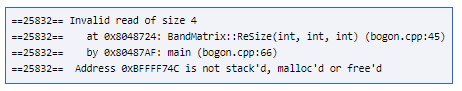
\includegraphics[width=0.8\textwidth]{errorReporting.png}
%  \caption{Primer izlaza alta Memcheck, izvor: \cite{ValgrindCore}}
%  \label{fig:slika2.1}
%\end{figure}

\begin{lstlisting}[style=terminal,caption={Primer izlaza alta \textit{Memcheck} \cite{ValgrindCore}}, label={lst:slika2.1},language={bash}]   
==25832==  Invalid read of size 4
==25832==      at 0x8048724: BandMatrix::ReSize(int, int, int) (bogon.cpp:45)
==25832==      by 0x80487AF: main (bogon.cpp:66)
==25832==  Address 0xBFFFF74C is not stack'd, malloc'd or free'd
\end{lstlisting}

Ova poruka kaže da je program izvršio ilegalno 4-bajtno čitanje adrese 0xBFFFF74C, koja nije važeća adresa steka niti odgovara bilo kojem trenutnom bloku hipa ili nedavno oslobođenim blokovima hipa. Čitanje se događa u redu 45 \textit{bogon.cpp}, pozvanog iz reda 66 iste datoteke. Za greške povezane sa identifikovanim (trenutnim ili oslobođenim) blokom hipa, npr. čitanje oslobođene memorije, \textit{Valgrind} izveštava ne samo o lokaciji na kojoj se dogodila greška, već i gde je pridruženi blok hipa dodeljen/oslobođen.

\textit{Valgrind} pamti sve izveštaje o greškama. Kada se otkrije greška, ona se upoređuje sa starim izveštajima da bi se videlo da li je duplikat. Ako je tako, greška je zabeležena, ali dalji komentari se ne emituju. Na ovaj način, alat izbegava zatrpavanje velikim brojem duplikata izveštaja o greškama.  

Zanimljivo je da se greške prijavljuju pre nego što se pridružena operacija zaista dogodi. Na primer, ako se koristi \textit{Memcheck} i program pokušava da čita sa adrese nula, \textit{Memcheck} će poslati poruku u tom smislu, a program će onda verovatno zaustaviti rad sa greškom \textit{Segmentation fault}. Generalno, dobra je praksa ispravljati greške redosledom u kojem su prijavljene. Ukoliko se ne primeni pomenuta praksa, to može da zbuni. Na primer, program koji kopira neinicijalizovane vrednosti na nekoliko memorijskih lokacija i kasnije ih koristi, generisaće nekoliko poruka o grešci kada se pokrene na \textit{Memcheck}-u. Prva takva poruka o grešci može sasvim direktno dati osnovni uzrok problema. 

Proces otkrivanja duplikata grešaka prilično je skup i može prouzrokovati značajno usporenje ako program generiše ogromne količine grešaka. Da bi izbegao ozbiljnije probleme, \textit{Valgrind} će jednostavno zaustaviti prikupljanje grešaka nakon što uoči 1.000 različitih grešaka ili ukupno 10.000.000 grešaka. U ovoj situaciji potrebno je zaustaviti program i popraviti ga, jer \textit{Valgrind} neće prijaviti ništa drugo nakon ovoga. Ograničenja od 1.000 / 10.000.000 primenjuju se nakon uklanjanja potisnutih grešaka, odnosno onih grešaka za koje \textit{Memcheck} utvrdi da su duplikati. Ova ograničenja su definisana u \textit{m\_errormgr.c} i mogu se povećati ako je potrebno \cite{ValgrindCore}. 

\section{Memcheck}
\textit{Memcheck} je alat koji vrši detekciju grešaka u radu sa memorijom \cite{Memcheck}. Može da otkrije sledeće probleme koji su česti u programima C i C ++:
\begin{itemize}
\item Pristup memoriji kojoj ne biste smeli, tj.~prekoračenje i potkoračenje blokova hipa, prekoračenje vrha steka i pristup memoriji nakon što se oslobodi.
\item Korišćenje nedefinisanih vrednosti, tj.~vrednosti koje nisu inicijalizovane ili su izvedene iz drugih nedefinisanih vrednosti.
\item Pogrešno oslobađanje memorije hipa, poput dvostrukog oslobađanja blokova hipa, ili neusklađena upotreba \textit{malloc/new/new[]} naspram \textit{free/ delete/delete[]}.
\item Preklapanje \textit{src} i \textit{dst} pokazivača u \textit{memcpy} i srodnim funkcijama.
\item Prosleđivanje sumnjive (verovatno negativne) vrednosti parametru veličine funkcije dodeljivanja memorije.
\item Curenje memorije.
\end{itemize}

Problemi poput ovih teško se mogu pronaći drugim sredstvima, često ostajući neotkriveni tokom dužih perioda, a zatim uzrokujući povremene padove, čiji je pravi razlog obično teško uočljiv. Upravo iz tih razloga memorijske greške spadaju u grupu najteže detektujućih grešaka pa je samim tim i njihovo otklanjanje težak zadatak.

Kao što je rečeno u prethodnoj sekciji, da bi se dobile detaljne, a pritom i neophodne informacije o programu, koristeći \textit{Memcheck}, program treba kompajlirati sa uključenom opcijom \texttt{-g}. Što se optimizacije tiče, prilikom korišćenja alata \textit{Memcheck}, u retkim prilikama, primećeno je da su optimizacije kompajlera (optimizacija \texttt{-O2} i više optimizacije, a ponekad čak i optimizacija \texttt{-O1}) generisale k\^od koji zavara \textit{Memcheck} da pogrešno prijavljuje greške vezane za neinicijalizovane vrednosti \cite{ValgrindCore}. Razvojni tim \textit{Valgrind}-a je detaljno razmotrio kako to popraviti i nažalost došli su do rezultata da bi popravljanje te greške dovelo do značajnog usporavanja alata. Dakle, najbolje rešenje je potpuno isključiti optimizaciju. Budući da ovo često stvari čini nekontrolisano sporima, razuman kompromis je korišćenje opcije \texttt{-O0}. Ovo donosi većinu prednosti viših nivoa optimizacije, dok istovremeno ima relativno male šanse za lažno pozitivne ili lažno negativne podatke od \textit{Memcheck}-a. Takođe, poželjno je kompajlirati k\^od sa \texttt{-Wall} jer on može identifikovati neke ili sve probleme koje \textit{Valgrind} može propustiti na višim nivoima optimizacije. Nivo optimizacije ne utiče na sve ostale alate, a za alate za profajliranje kao što je \textit{Cachegrind} bolje je da program kompajlirate na normalnom nivou optimizacije \cite{ValgrindCore}. 

% (Korišćenje \texttt{-Wall} je takođe dobra ideja u celini.)

Da biste koristili ovaj alat, možete da navedete opciju \texttt{--tool = memcheck} u komandnoj liniji prilikom pokretanja \textit{Valgrind}-a, ali niste u obavezi s obzirom da je \textit{Memcheck} podrazumevani alat.
 \begin{center}
\texttt{valgrind –tool=memcheck [argumenti memchecka] program [argumenti programa]}
\end{center}

Program koji radi pod kontrolom \textit{Memcheck}-a obično je deset do pedeset puta sporiji nego kada se izvršava samostalno, što je posledica translacije koda \cite{ValgrindCore}. Više o tome biće rečeno u sekciji koja sledi. Izlaz iz programa biće povećan za izlaz koji daje \textit{valgrind} i sam alat \textit{Memcheck}, koji se ispisuje na standardnom izlazu za greške ukoliko se ne definiše drugačije \cite{ValgrindDOC}. 

\subsection{Princip funkcionisanja alata Memcheck}

U ovoj sekciji biće opisani mehanizmi koje \textit{Memcheck} koristi u detektovanju grešaka, nakon čega će biti obrađene greške koje može detektovati.

\subsubsection{Bitovi valjane vrednosti (V bitovi)}
Najjednostavnije je razmišljati o \textit{Memcheck}-u kao alatu koji implementira sintetički CPU koji je identičan stvarnom CPU, osim jednog ključnog detalja. Svaki bit (doslovno) podataka koje obrađuje, čuva i njima rukuje stvarni CPU, dok u sintetičkom CPU ima pridruženi bit ,,valjane vrednosti'' (eng. \textit{valid-value bit}), koji govori da li prateći bit ima legitimnu vrednost ili ne. U daljem tekstu ovaj bit se naziva \texttt{V} bitom (valjane vrednosti).

Svaki bajt u sistemu iz tog razloga ima i 8\texttt{V} bitova koji ga prate. Na primer, kada CPU učita reč veličine 4 bajta iz memorije, takođe učitava odgovarajućih 32\texttt{V} bita iz bitmape koja čuva \texttt{V} bitove za čitav adresni prostor procesa. Ako bi CPU kasnije trebalo da upiše celu ili neki deo te vrednosti u memoriju na drugoj adresi, relevantni V bitovi će se sačuvati nazad u \texttt{V}-bitnoj bitmapi.

Ukratko, svaki bit u sistemu ima (konceptualno) pridruženi \texttt{V} bit, koji ga prati svuda, čak i unutar CPU-a. Svi registri CPU-a (celi brojevi, registri za brojeve u pokretnom zarezu, vektori i uslovi) imaju svoje \texttt{V} bitne vektore. Da bi ovo moglo da funkcioniše dovoljno efikasno, \textit{Memcheck} koristi veliku količinu kompresije da bi kompaktno prikazao \texttt{V} bitove.

Kopiranje vrednosti ne dovodi do toga da \textit{Memcheck} proverava greške ili izveštava o njima. Međutim, kada se vrednost koristi na način koji bi mogao da utiče na spoljno-vidljivo ponašanje programa, pridruženi \texttt{V} bitovi se tada proveravaju. Ako bilo koji od njih ukazuje da je vrednost nedefinisana (odnosno promenljiva definisana ali neinicijalizovana), čak i delimično, prijaviće se greška.

Većina operacija na niskom nivou, kao što je sabiranje, uzrokuje da \textit{Memcheck} koristi \texttt{V} bitove za operande za izračunavanje \texttt{V} bitova za rezultat. Čak i ako je rezultat delimično ili u potpunosti nedefinisan, alat ne prijavljuje grešku. Provere definisanosti dešavaju se samo na tri mesta:
\begin{itemize}
\item  kada se vrednost koristi za generisanje memorijske adrese;
\item  kada treba doneti odluku o kontroli toka izvršavanja programa; 
\item  kada se detektuje sistemski poziv, u kom slučaju će \textit{Memcheck} proveravati definisanost parametara prema potrebi.
\end{itemize}

Kada provera detektuje nedefinisanost, izdaje se poruka o grešci. Dobijena vrednost se na dalje smatra dobro definisanom, kako bi se izbegli dugi lanci poruka o greškama. Drugim rečima, kada \textit{Memcheck} prijavi grešku nedefinisane vrednosti, pokušava da izbegne prijavljivanje daljih grešaka izvedenih iz te iste nedefinisane vrednosti. Ideja o proveravanju svih čitanja iz memorije i žalbi ukoliko je nedefinisana vrednost učitana u registar procesora ne funkcioniše dobro, jer savršeno legitimni C programi rutinski kopiraju neinicijalizovane vrednosti u memoriji, što bi u slučaju primene pomenute ideje dovelo do enormno velikog broja prijavljenih grešaka. Primer sa listinga \ref{lst:slika2.2} ilustruje tu problematiku.

\begin{lstlisting}[style=mystyle,caption={Primer kratkog segmenta koda}, label={lst:slika2.2},language={C}] 
struct S{
	int x;
	char c;
};

struct S s1, s2;
s1.x = 2020;
s1.c = 'a';
s2=s1;
\end{lstlisting}

%\begin{figure}[!ht]
%  \centering
%  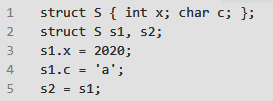
\includegraphics[width=0.5\textwidth]{picture2.2.png}
%  \caption{Primer kratkog segmenta koda}
%  \label{fig:slika2.2}
%\end{figure}

Nakon analize koda sa listinga \ref{lst:slika2.2}, može da deluje da struktura \texttt{S}, kako tip podataka \texttt{int} zauzima 4 bajta, a tip podataka \texttt{char} jedan bajt, zauzima 5 bajtova. Međutim, svi kompajleri, u normalnom režimu rada, zaokružiće veličinu strukture \texttt{S} na ceo broj reči, tj.~na 8 bajtova. Dakle, \texttt{s1} zauzima 8 bajtova, ali će samo njih 5 biti inicijalizovano. Za zadatak \texttt{s2=21}, GCC generiše k\^od za kopiranje svih 8 bajtova u \texttt{s2} bez obzira na njihovo značenje. Ako bi \textit{Memcheck} jednostavno proveravao vrednosti redom kako su izašle iz memorije, oglasio bi svaki put kad bi se desilo ovakvo dodeljivanje strukture. Dakle, neophodno je komplikovanije ponašanje opisano gore. Ovo omogućava GCC-u da kopira \texttt{s1} u \texttt{s2} na bilo koji način, a upozorenje će se emitovati samo ako se kasnije koriste neinicijalizovane vrednosti \cite{Memcheck}. 

\subsubsection{Bitovi važeće adrese (A bitovi)}
Prethodna sekcija opisuje kako se uspostavlja i održava valjanost vrednosti bez potrebe da se kaže da li program ima ili nema pravo na pristup bilo kojoj određenoj memorijskoj lokaciji. U ovoj sekciji ćemo razmotriti to pitanje.

Svaki bit u memoriji ili u procesoru ima pridruženi bit valjane vrednosti (\texttt{V}). Pored toga, svi bajtovi u memoriji, ali ne i u procesoru, imaju pridruženi bit valjane adrese (\texttt{A}, eng. \textit{valid-address bit}). Ovo ukazuje na to da li program može legitimno čitati ili pisati u tu lokaciju. To ne daje nikakve naznake valjanosti podataka na toj lokaciji, kako je to zadatak V bitova već samo da li se toj lokaciji može pristupiti ili ne. Svaki put kada program čita ili upisuje u memoriju, \textit{Memcheck} proverava \texttt{A} bitove povezane sa adresom. Ako bilo koji od njih označi neispravnu adresu, prijavljuje se greška. Sama čitanja i pisanja ne menjaju \texttt{A} bitove, već ih samo konsultuju. Ovaj naizgled čudan izbor smanjuje količinu zbunjujućih informacija koje se predstavljaju korisniku. Izbegava neprijatnu pojavu u kojoj se memorija čita sa mesta koje je i nedostupno i sadrži nevažeće vrednosti, a kao rezultat toga dobila bi se ne samo greška sa nevažećom adresom (čitanje / pisanje), već i potencijalno veliki skup greškaka neinicijalizovanih vrednosti --- jedna za svaki put kada se vrednost koristi.

Princip postavljanja, odnosno čišćenja \texttt{A} bitova je sledeći:
\begin{itemize}
\item Kada se program pokrene, sva globalna područja podataka su označena kao pristupačna.
\item Kada program izvrši \textit{malloc/new}, A bitovi za tačno dodeljeno područje označeni su kao pristupačni. Po oslobađanju područja A bitovi se menjaju kako bi ukazali na nepristupačnost.
\item Kada se registar pokazivača steka (SP) pomeri gore ili dole, postavljaju se \texttt{A} bitovi. Pravilo je da je područje SP od vrha do podnožja steka označeno kao pristupačno, a ispod SP nepristupačno. 
%(Ako to zvuči nelogično, imajte na umu da stek raste prema dole, a ne prema gore, na gotovo svim Unix sistemima, uključujući GNU / Linux.) 
\item Pri obavljanju sistemskih poziva, \texttt{A} bitovi se odgovarajuće menjaju. Na primer, \textit{mmap} čini da se datoteke pojavljuju u adresnom prostoru procesa, pa se \texttt{A} bitovi moraju ažurirati ako \textit{mmap} uspe \cite{Memcheck}. 
\end{itemize}

Nakon svega navedenog dolazimo do rezimea \textit{Memcheck}-ovog principa funkcionisanja.
\begin{itemize}
\item[$\textendash$] Svaki bajt u memoriji ima 8 pridruženih \texttt{V} bitova (važeće vrednosti), govoreći da li bajt ima definisanu vrednost i jedan bit \texttt{A} (valjane adrese), odnosno govoreći da li program trenutno ima pravo da čita/piše na tu adresu. Kao što je gore pomenuto, velika upotreba kompresije omogućava da troškovi obično iznose oko 25\% vremena i prostora.
\item[$\textendash$] Kada se memorija čita ili se u nju piše, pregledaju se odgovarajući \texttt{A} bitovi. Ako označe nevažeću adresu, \textit{Memcheck} emituje grešku \textit{neispravno čitanje} (eng. \textit{invalid read}) ili \textit{neispravno pisanje} (eng. \textit{invalid write}).
\item[$\textendash$] Kada se memorija čita u registre CPU-a, relevantni \texttt{V} bitovi se preuzimaju iz memorije i čuvaju u simuliranom CPU-u. Oni se ne konsultuju.
\item[$\textendash$] Kada se registar ispiše u memoriju, V bitovi za taj registar se takođe zapisuju nazad u memoriju.
\item[$\textendash$] Kada se vrednosti u registrima CPU koriste za generisanje memorijske adrese ili za određivanje ishoda uslovne grane, \texttt{V} bitovi za te vrednosti se proveravaju i emituje se greška ako je bilo koja od njih nedefinisana. Kada se vrednosti u registrima procesora koriste u bilo koju drugu svrhu, \textit{Memcheck} izračunava \texttt{V} bitove za rezultat, ali ih ne proverava.
\item[$\textendash$] Jednom kada se provere \texttt{V} bitovi za vrednost u CPU, oni se postavljaju da ukazuju na validnost. Ovo izbegava dugačke lance grešaka.
\item[$\textendash$] Kada se vrednosti učitaju iz memorije, \textit{Memcheck} proverava \texttt{A} bitove za tu lokaciju i izdaje upozorenje o nevalidnoj adresi ako je potrebno. U tom slučaju su učitani \texttt{V} bitovi primorani da označe validno stanje, uprkos tome što je lokacija nevalidna. 
\item[$\textendash$] \textit{Memcheck} presreće pozive funkcija \textit{malloc, calloc, realloc, valloc, memalign, free, new, new[], delete i delete[]}. Ponašanje koje  se dobija usled toga je sledeće:
	\begin{itemize}
	\item[$\textbullet$] \textit{malloc/new/new[]}: vraćena memorija je označena kao adresabilna, ali nema važeće vrednosti. To znači da u nju morate pisati pre nego što je pročitate.
	\item[$\textbullet$] \textit{calloc}: vraćena memorija označena je i adresabilnom i važećom, jer \textit{calloc} postavlja područje na nulu.
	\item[$\textbullet$] \textit{realloc}: ako je nova veličina veća od stare, novi odeljak je adresiran, ali nevažeći, kao kod \textit{malloc}-a. Ako je nova veličina manja, odloženi odeljak je označen kao nedostupan. \textit{Realloc}-u može da se prosledi bilo šta, ali ispravno je samo ako se prosledi pokazivač koji je prethodno izdao \textit{malloc/calloc/realloc}.
	\item[$\textbullet$] \textit{free/delete/delete[]}: ovim funkcijama može se proslediti samo pokazivač koji je prethodno izdala odgovarajuća funkcija dodeljivanja. Inače, \textit{Memcheck} prijavljuje nepravilnost. Ako je pokazivač zaista važeći, \textit{Memcheck} označava celo područje na koje pokazuje kao da ga nije moguće adresirati i postavlja blok u red oslobođenih blokova. Cilj je odložiti što je duže moguće realokaciju ovog bloka. Dok se to ne dogodi, svi pokušaji da mu se pristupi izazvaće grešku nevažeće adrese \cite{ValgrindDOC}. 
	\end{itemize}
\end{itemize}

\subsection{Greške nevalidnog čitanja/pisanja (eng. \textit{invalid read/write errors})}
%\begin{figure}[!ht]
%  \centering
%  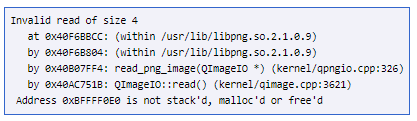
\includegraphics[width=0.7\textwidth]{invalidReadError.png}
%  \caption{Primer ispisa greške nevalidnog čitanja, izvor: \cite{Memcheck}}
%  \label{fig:slika2.3}
%\end{figure}

\begin{lstlisting}[style=terminal,caption={Primer ispisa greške nevalidnog čitanja \cite{Memcheck}}, label={lst:slika2.3},language={bash}]   
Invalid read of size 4
    at 0x40F6BBCC: (within /usr/lib/libpng.so.2.1.0.9)
    by 0x40F6B804: (within /usr/lib/libpng.so.2.1.0.9)
    by 0x40B07FF4: read_png_image(QImageIO *) (kernel/qpngio.cpp:326)
    by 0x40AC751B: QImageIO::read() (kernel/qimage.cpp:3621)
Address 0xBFFFF0E0 is not stack'd, malloc'd or free'd
\end{lstlisting}

Ove greške se javljaju kada program čita ili piše u memoriju na mestu za koje \textit{Memcheck} smatra da ne bi trebalo. U ovom primeru, program je izvršio četvorobajtno čitanje na adresi 0xBFFFF0E0, negde unutar sistemske biblioteke \textit{libpng.so.2.1.0.9}, koja je pozvana negde drugde u istoj biblioteci, a koje je izvšeno iz linije 326 u okviru fajla \textit{qpngio.cpp} , i tako dalje.

\textit{Memcheck} će svakako pokušati da odredi na šta se ilegalna adresa može odnositi, jer je to često korisno. Dakle, ako pokazuje na blok memorije koji je već oslobođen, alat će emitovati tu informaciju, kao i podatak o tome gde je blok oslobođen. Isto tako, ako se ispostavi da se nalazi na kraju hip bloka, što je greška, tj.~greška prekoračenja niza, alat će i to registrovati i prijaviiti, kao i podatak o tome gde je blok dodeljen. Ako koristite opciju \texttt{--read-var-info}, \textit{Memcheck} će raditi sporije, ali može dati detaljniji opis bilo koje nelegalne adrese.

U ovom primeru \textit{Memcheck} ne može da identifikuje adresu. Zapravo se adresa nalazi na steku, ali iz nekog razloga ovo nije važeća adresa steka - nalazi se ispod pokazivača steka i to nije dozvoljeno. U ovom konkretnom slučaju greška je verovatno uzrokovana GCC-om koji generiše nevažeći k\^od, što je poznata greška u nekim drevnim verzijama GCC-a.

Treba imati na umu da \textit{Memcheck} samo govori da će program uskoro pristupiti memoriji na nedozvoljenoj adresi i da pritom taj pristup ne može sprečiti. Dakle, kada program pristupi, što bi obično rezultiralo greškom (eng. \textit{Segmentation fault}), program će i dalje imati isto ponašanje - ali \textit{Memcheck}-a će izdati poruku neposredno pre toga. U ovom konkretnom primeru čitanje loših (nevalidnih) vrednosti sa steku nije fatalno, i program nastavlja sa radom \cite{ValgrindDOC}. 

\subsection{Korišćenje neinicijalizovanih vrednosti}
Greška pri korišćenju neinicijalizovane vrednosti se prijavljuje kada program koristi vrednost koja nije inicijalizovana - drugim rečima, nije definisana. Ovde se nedefinisana vrednost koristi negde unutar funkcije \texttt{printf} iz standardne C biblioteke. Ova greška je prijavljena prilikom pokretanja programa sa listinga \ref{lst:slika2.4}, dok je njen ispis dat na listingu \ref{lst:slika2.5}.

\begin{lstlisting}[style=mystyle,caption={Program koji izaziva grešku korišćenja neinicijalizovanih vrednosti}, label={lst:slika2.4},language={C}] 
#include <stdio.h>
#include <stdlib.h>

int main(){
	int x;
	printf("%d\n", x);
	exit(EXIT_SUCCESS);
}
\end{lstlisting}

%\begin{figure}[!ht]
%  \centering
%  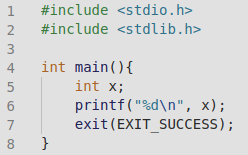
\includegraphics[width=0.5\textwidth]{uninitialisedErrorProgram.png}
%  \caption{Program koji izaziva grešku korišćenja neinicijalizovanih vrednosti}
%  \label{fig:slika2.4}
%\end{figure}

%\begin{figure}[!ht]
%  \centering
%  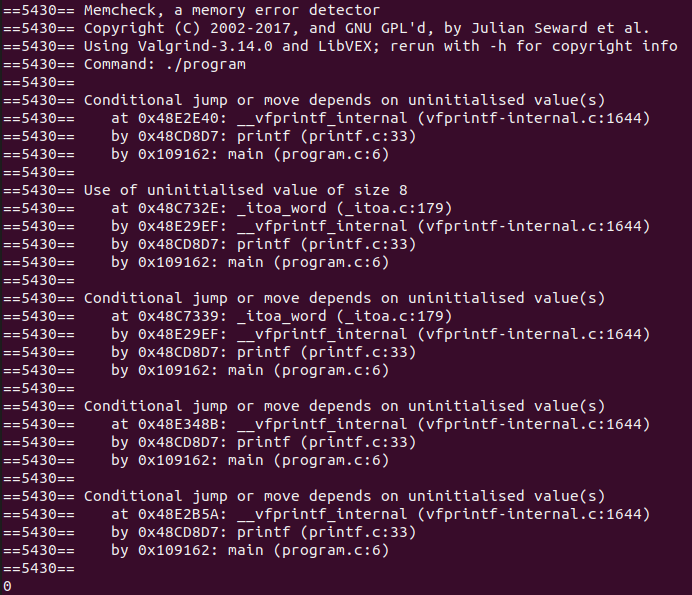
\includegraphics[width=0.7\textwidth]{uninitialisedError.png}
%  \caption{Primer ispisa greške korišćenja neinicijalizovanih vrednosti}
%  \label{fig:slika2.5}
%\end{figure}

\begin{lstlisting}[style=terminal,caption={Primer ispisa greške korišćenja neinicijalizovanih vrednosti}, label={lst:slika2.5},language={bash}] 
==5430== Memcheck, a memory error detector
==5430== Copyright (C) 2002-2017, and GNU GPL'd, by Julian Seward et al. 
==5430== Using Valgrind-3.14.0 and LibVEX; rerun with -h for copyright info 
==5430== Command: ./program
==5430==
==5430== Conditional jump or move depends on uninitialised value(s)
==5430==	at 0x48E2E40: __vfprintf_internal (vfprintf-internal.c:1644)
==5430==	by 0x48CD8D7: printf (printf.c:33)
==5430==	by 0x109162: main (program.c:6)
==5430==
==5430== Use of uninitialised value of size 8
==5430==	at 0x48C732E: _itoa_word (_itoa.c:179)
==5430==	by 0x48E29EF: __vfprintf_internal (vfprintf-internal.c:1644)
==5430==	by 0x48CD8D7: printf (printf.c:33)
==5430==	by 0x109162: main (program.c:6)
==5430==
==5430== Conditional jump or move depends on uninitialised value(s)
==5430==	at 0x48C7339: _itoa_word (_itoa.c:179)
==5430==	by 0x48E29EF: __vfprintf_internal (vfprintf-internal.c:1644)
==5430==	by 0x48CD8D7: printf (printf.c:33)
==5430==	by 0x109162: main (program.c:6)
==5430==
==5430== Conditional jump or move depends on uninitialised value(s)
==5430==	at 0x48E348B: __vfprintf_internal (vfprintf-internal.c:1644)
==5430==	by 0x48CD8D7: printf (printf.c:33)
==5430==	by 0x109162: main (program.c:6)
==5430==
==5430== Conditional jump or move depends on uninitialised value(s)
==5430==	at 0x48E2B5A: __vfprintf_internal (vfprintf-internal.c:1644)
==5430==	by 0x48CD8D7: printf (printf.c:33)
==5430==	by 0x109162: main (program.c:6)
==5430==
0
\end{lstlisting}

%Važno je shvatiti da program može kopirati neželjene (neinicijalizovane) podatke koliko god želi. \textit{Memcheck} to posmatra i evidentira podatke, ali se ne žali.
Poruka o grešci se izdaje samo kada program pokušava da koristi neinicijalizovane podatke na način koji može uticati na spolja vidljivo ponašanje programa, iako \textit{Memcheck} prati i evidentira svako korišćenje neinicijalizovanih podataka. U ovom primeru, \textit{x} je neinicijalizovano. \textit{Memcheck} primećuje vrednost koja se prosleđuje \textit{\_IO\_printf} i odatle \textit{\_IO\_vfprintf}, ali ne daje komentar. Međutim, \textit{\_IO\_vfprintf} mora ispitati vrednost  kako bi je mogao pretvoriti u odgovarajući ASCI niz i \textit{Memcheck} u ovom trenutku prijavljuje grešku.

Izvori grešaka neinicijalizovanih vrednosti su sledeći:
\begin{itemize}
\item Lokalne promenljive u procedurama koje nisu inicijalizovane, kao u primeru sa listinga \ref{lst:slika2.4}.
\item Sadržaj blokova hipa (dodeljen \textit{malloc}-om, \textit{new} ili sličnom funkcijom) pre nego što se nešto u tom bloku ispiše, odnosno pre inicijalizacije.
\end{itemize}

Za dobijanje informacija o izvorima neinicijalizovanih podataka u programu, neophodno je koristiti opciju \texttt{--track-origins=yes}. Ovo čini \textit{Memcheck} sporijim, ali može znatno olakšati pronalaženje osnovnih uzroka neinicijalizovanih grešaka \cite{Memcheck}. 

\subsection{Korišćenje neinicializovane ili neadresirane vrednosti u sistemskom pozivu}

\textit{Memcheck} prati i proverava sve parametre sistemskih poziva. Svaki parametar se proverava pojedinačno, bio on inicijalizovan ili ne. Ukoliko sistemski poziv treba da čita iz bafera  koji je obezbeđen programu, \textit{Memcheck} proverava da li je ceo bafer adresiran i da li je njegov sadržaj inicijalizovan. Takođe, ako sistemski poziv treba da piše u bafer, \textit{Memcheck} proverava da li je bafer moguće adresirati. Nakon sistemskog poziva, \textit{Memcheck} ažurira sve parametre koje je pratio kako bi tačno odražavale sve promene u stanju memorije izazvane sistemskim pozivom.

\begin{lstlisting}[style=mystyle,caption={Program koji izaziva grešku korišćenja neinicializovane ili neadresirane vrednosti u sistemskom pozivu \cite{Memcheck}}, label={lst:slika2.6},language={C}] 
#include <unistd.h>
#include <stdlib.h>

int main(void){
	char* arr = malloc(10);
	int *arr2 = malloc(sizeof(int));
	write(1 /* stdout */, arr, 10);
	exit(arr2[0]);
}
\end{lstlisting}

%\begin{figure}[!ht]
%  \centering
%  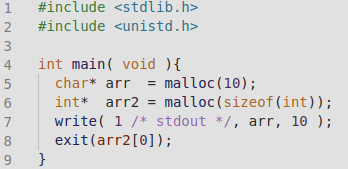
\includegraphics[width=0.5\textwidth]{sysCallErrorProgram.png}
%  \caption{Program koji izaziva grešku korišćenja neinicializovane ili neadresirane vrednosti u sistemskom pozivu, izvor: \cite{Memcheck}}
%  \label{fig:slika2.6}
%\end{figure}

%\begin{figure}[!ht]
 % \centering
%  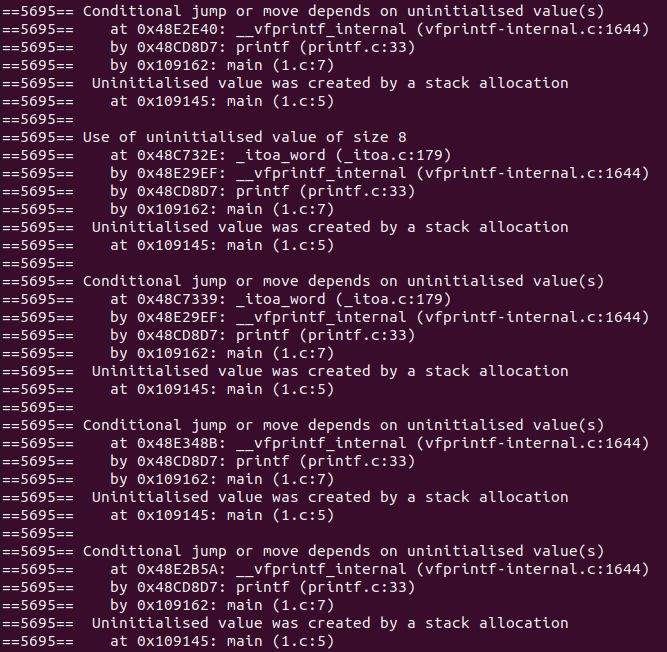
\includegraphics[width=0.7\textwidth]{sysCallError.png}
%  \caption{Primer ispisa greške korišćenja neinicializovane ili neadresirane vrednosti u sistemskom pozivu}
%  \label{fig:slika2.7}
%\end{figure}

\begin{lstlisting}[style=terminal,caption={Primer ispisa greške korišćenja neinicializovane ili neadresirane vrednosti u sistemskom pozivu}, label={lst:slika2.7},language={bash}] 
Syscall param write(buf) points to uninitialised byte(s)
   at 0x25A48723: __write_nocancel (in /lib/tls/libc-2.3.3.so)
   by 0x259AFAD3: __libc_start_main (in /lib/tls/libc-2.3.3.so)
   by 0x8048348: (within /auto/homes/njn25/grind/head4/a.out)
 Address 0x25AB8028 is 0 bytes inside a block of size 10 alloc'd
   at 0x259852B0: malloc (vg_replace_malloc.c:130)
   by 0x80483F1: main (a.c:5)

Syscall param exit(error_code) contains uninitialised byte(s)
   at 0x25A21B44: __GI__exit (in /lib/tls/libc-2.3.3.so)
   by 0x8048426: main (a.c:8)
\end{lstlisting}

Na listinzima \ref{lst:slika2.6} i \ref{lst:slika2.7} dat je primer programa koji ilustruje sistemski poziv sa neispravnim parametrima, kao i izveštaj koji dobijamo nakon analize pomenutog programa. Sa listinga \ref{lst:slika2.7} vidimo da je \textit{Memcheck} prikazao dve greške sa informacijama o korišćenju neinicijalizovanih vrednosti u sistemskim pozivima, kao i linije izvornog koda gde se ove vrednosti koriste. Prva greška posledica je korišćenja neinicijalizovane vrednosti \textit{arr} kao paramatra sistemskog poziva \textit{write()}, dok je druga greška posledica prosleđenog nedefinisanog argumenta sistemskom pozivu \textit{exit} \cite{Memcheck}. 

\subsection{Nedopušteno oslobađanje memorije}
\textit{Memcheck} prati sve blokove memorije koje je program alocirao pomoću \textit{malloc/new}, tako da može tačno znati da li je argument prosleđen \textit{free/ delete} legitiman ili ne. Listing \ref{lst:slika2.8} ilustruje program koji je oslobodio isti blok dva puta. 

\begin{lstlisting}[style=mystyle,caption={Program koji oslobađa isti blok dva puta}, label={lst:slika2.8},language={C}] 
#include <stdio.h>
#include <stdlib.h>

int main(){
	char *p;
	p = (char) malloc(5);
	p = (char) malloc(7);
	free(p);
	free(p);
	p = (char) malloc(9);
	exit(EXIT_SUCCESS);
}
\end{lstlisting}

%\begin{figure}[!ht]
%  \centering
%  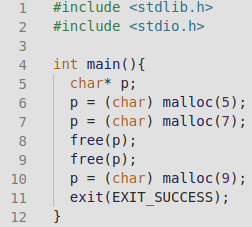
\includegraphics[width=0.5\textwidth]{invalidFreeErrorProgram.png}
%  \caption{Program koji oslobađa isti blok dva puta}
%  \label{fig:slika2.8}
%\end{figure}

Kao i kod grešaka nevalidnog čitanja/pisanja, \textit{Memcheck} pokušava da dokuči oslobođenu adresu. Ako je, kao ovde, slučaj da je adresa koja je prethodno oslobođena, to će biti prijavljeno i učiniće duplikate oslobađanja istog bloka lako uočljivim. Ova poruka će biti emitovana i ako program pokuša da oslobodi pokazivač koji ne pokazuje na početak hip bloka. Listing \ref{lst:slika2.9} ilustruje izlaz dobijen puštanjem programa sa listinga \ref{lst:slika2.8} na analizu alatom \textit{Memcheck} \cite{Memcheck}. 

%\begin{figure}[!ht]
%  \centering
%  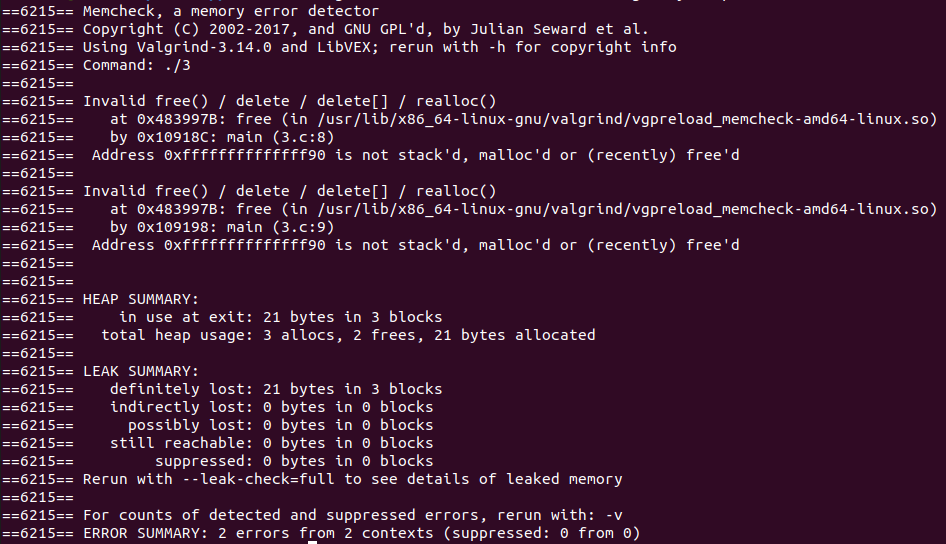
\includegraphics[width=0.7\textwidth]{invalidFreeError.png}
%  \caption{Primer ispisa greške nedopuštenog oslobađanja memorije}
%  \label{fig:slika2.9}
%\end{figure}

\begin{lstlisting}[style=terminal,caption={Primer ispisa greške nedopuštenog oslobađanja memorije}, label={lst:slika2.9},language={bash}] 
==6215==  Memcheck, a memory error detector
==6215==  Copyright (C) 2002-2017, and GNU GPL'd, by Julian Seward et al. Using Valgrind-3.14.0 and LibVEX; rerun with -h for copyright info 
==6215==  Command: ./3
==6215== 
==6215==  Invalid free() / delete / delete[] / realloc()
==6215==     at 0x483997B: free (in /usr/lib/x86_64-linux-gnu/valgrind/vgpreload_memcheck-amd64-linux.so) 
==6215==     by Ox10918C: main (3.c:8)
==6215==  Address Oxffffffffffffff90 is not stack'd, malloc'd or (recently) free'd
==6215== 
==6215==  Invalid free() / delete / delete[] / realloc()
==6215==     at 0x483997B: free (in /usr/ltb/x86_64-linux-gnu/valgrind/vgpreload_memcheck-amd64-linux.so) 
==6215==     by 0x109198: main (3.c:9)
==6215==  Address Oxffffffffffffff9O is not stack'd, malloc'd or (recently) free'd
==6215== 
==6215==   HEAP SUMMARY:
==6215==       in use at exit: 21 bytes in 3 blocks
==6215==       total heap usage: 3 allocs, 2 frees, 21 bytes allocated
==6215== 
==6215==   LEAK SUMMARY:
==6215==      definitely lost: 21 bytes in 3 blocks 
==6215==      indirectly lost: 0 bytes in 0 blocks
==6215==      possibly lost: 0 bytes in 0 blocks 
==6215==      still reachable: 0 bytes in 0 blocks
==6215==      suppressed: 0 bytes in 0 blocks
==6215==  Rerun with --leak-check=full to see details of leaked memory
==6215==  For counts of detected and suppressed errors, rerun with: -v 
==6215==  ERROR SUMMARY: 2 errors from 2 contexts (suppressed: 0 from 0)
\end{lstlisting}

\subsection{Preklapanje izvornog i odredišnog bloka}
Sledeće bibliotečke funkcije kopiraju neke podatke iz jednog memorijskog bloka u drugi - \textit{memcpy, strcpy, strncpy, strcat, strncat}.  Blokovi na koje ukazuju njihovi pokazivači \textit{src} i \textit{dst} ne smeju se preklapati. \textit{POSIX} standardi imaju sledeću formulaciju: ,,Ako se kopiranje vrši između objekata koji se preklapaju, ponašanje je nedefinisano''.  Stoga \textit{Memcheck} ovo proverava. Ukoliko dođe do preklapanja, prijaviće grešku.
%\begin{figure}[!ht]
 % \centering
%  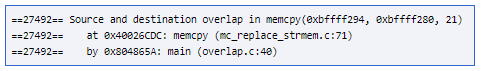
\includegraphics[width=0.7\textwidth]{overlapError.png}
%  \caption{Primer ispisa greške preklapanja izvornog i odredišnog bloka, izvor: \cite{Memcheck}}
%  \label{fig:slika2.10}
%\end{figure}

\begin{lstlisting}[style=terminal,caption={Primer ispisa greške preklapanja izvornog i odredišnog bloka \cite{Memcheck}}, label={lst:slika2.10},language={bash}] 
==27492==  Source and destination overlap in memcpy(0xbffff294, 0xbffff280, 21)
==27492==      at 0x40026CDC: memcpy (mc_replace_strmem.c:71)
==27492==      by 0x804865A: main (overlap.c:40)
\end{lstlisting}

%Ne želite da se dva bloka preklapaju, jer bi jedan od njih mogao delimično da se prepiše kopiranjem. Može delovati da \textit{Memcheck} previše pedantno prijavljuje ovo u slučaju kada je \textit{dst} manji od \textit{src}. Na primer, očigledan način implementacije \textit{memcpy}  je kopiranje iz prvog bajta u poslednji. Međutim, vodiči za optimizaciju nekih arhitektura preporučuju kopiranje od poslednjeg bajta do prvog. Pouka priče je da ako zaista želite da napišete prenosivi k\^od, ne pravite nikakve pretpostavke o implentaciji jezika \cite{Memcheck}. 

\subsection{Sumnjive vrednosti argumenata}
Sve funkcije za alokaciju memorije uzimaju argument koji određuje veličinu memorijskog bloka koji treba dodeliti. Jasno je da tražena veličina treba da bude pozitivna vrednost koja obično nije preterano velika. Na primer, krajnje je neverovatno da veličina zahteva za dodelu premašuje ${2}^{63}$ bajta na 64-bitnoj mašini. Mnogo je verovatnije da je takva vrednost rezultat pogrešnog izračunavanja veličine i da je u stvari negativna vrednost (koja se čini preterano velikom jer se obrazac bita tumači kao neoznačeni celi broj). Takva vrednost se naziva ,,sumnjivom vrednošću''. Argument veličine sledećih funkcija dodeljivanja biće proveren da li je sumnjiv: \textit{malloc, calloc, realloc, memalign, new, new[ ], \_builtin\_new, \_builtin\_vec\_new}. Za \textit{calloc} se proveravaju oba argumenta.

Ukoliko dođe do ovakve situacije, prijaviće se greška sa listinga \ref{lst:slika2.11}. 
%\begin{figure}[!ht]
%  \centering
%  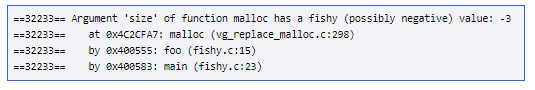
\includegraphics[width=0.7\textwidth]{fishyArgument.png}
%  \caption{Primer ispisa greške sumnjive vrednosti argumenata, izvor: \cite{Memcheck}}
 % \label{fig:slika2.11}
%\end{figure}

\begin{lstlisting}[style=terminal,caption={Primer ispisa greške sumnjive vrednosti argumenata \cite{Memcheck}}, label={lst:slika2.11},language={bash}] 
==32233==  Argument 'size' of function malloc has a fishy (possibly negative) value: -3
==32233==      at 0x4C2CFA7: malloc (vg_replace_malloc.c:298)
==32233==      by 0x400555: foo (fishy.c:15)
==32233==      by 0x400583: main (fishy.c:23)
\end{lstlisting}

\subsection{Detekcija curenja memorije}
Na kraju izvršavanja programa \textit{Memcheck} ima informaciju o svim blokovima hip memorije koji nisu oslobođeni, jer tokom izvršavanja programa \textit{Memcheck} vodi računa o svim blokovima hipa koji su alocirani. \textit{Memcheck} takođe može odrediti da li se svakom od tih blokova može pristupiti preko dostupnog pokazivača, ukoliko se na odgovarajući način podesi opcija \texttt{--leak-check} \cite{ValgrindDOC}.

Memorijskim blokovima se može pristupiti pomoću pokazivača. Postoje dve vrste pokazivača koje u tu svrhu koristimo:
\begin{itemize}
\item Pokazivač na početak memorijskog bloka (eng. \textit{start-pointer});
\item Pokazivač na sadržaj unutar memorijskog bloka (eng. \textit{interior-pointer}).
\end{itemize}

Ukoliko imamo pokazivač koji je pokazivao na početak bloka, koji je u međuvremenu pomeren da pokazuje na unutrašnjost bloka, ili postoji slučajna i nepovezana vrednost u memoriji koja pokazuje na unutrašnjost nekog memorijskog bloka, automatski znamo da imamo pokazivač na unutrašnjost memorijskog bloka. 

Imajući to na umu, na slici \ref{fig:slika2.12} navedeno je devet mogućih slučajeva kada pokazivači pokazuju na neke memorijske blokove.
\begin{figure}[!ht]
  \centering
  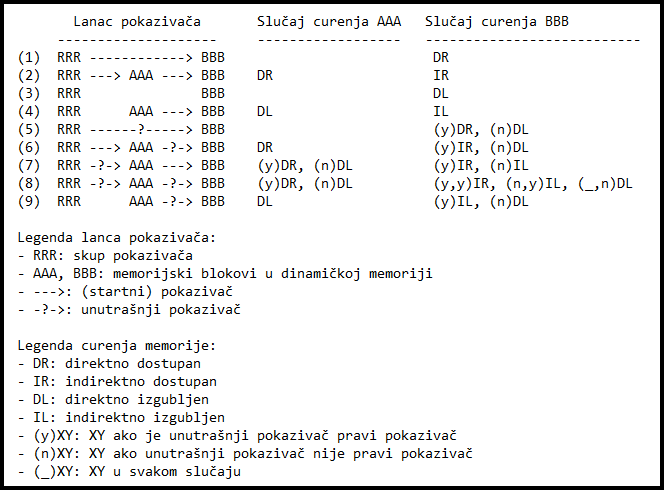
\includegraphics[width=0.8\textwidth]{memoryLeacking2.png}
  \caption{Primer pokazivača na memorijski blok}
  \label{fig:slika2.12}
\end{figure}


Svaki mogući slučaj može se svesti na jedan od gore navedenih devet. \textit{Memcheck} objedinjuje neke od ovih slučajeva, što rezultira u sledeće četiri kategorije curenja memorije.
\begin{itemize}
\item[$\textendash$] \textbf{Još uvek dostupan (eng. \textit{still reachable})} – Ova klasa pokriva slučajeve 1 i 2 navedene na slici \ref{fig:slika2.12}. Pronađen je pokazivač na početak bloka ili više takvih pokazivača. Kako ovi pokazivači pokazuju tačno na neoslobođeni segment memorije, isti se može osloboditi pre završetka rada programa. Blokovi iz ove kategorije su vrlo česti i verovatno nisu problem. Dakle, \textit{Memcheck} podrazumevano neće pojedinačno prijavljivati takve blokove \cite{ValgrindDOC}.
\item[$\textendash$] \textbf{Definitivno izgubljen (eng. \textit{definitely lost})} – Ova klasa pokriva slučaj 3 naveden na slici \ref{fig:slika2.12}. To znači da se ne može naći pokazivač na blok. Blok je klasifikovan kao ,,izgubljen'', jer oslobađanje istog nije moguće na izlazu iz programa, kako na njega ne postoji pokazivač. Ovo je verovatno simptom gubitka pokazivača u nekom ranijem trenutku programa. Takve slučajeve treba da popravi programer \cite{ValgrindDOC}.
\item[$\textendash$] \textbf{Indirektno izgubljen (eng. \textit{indirectly lost})} – Ova klasa pokriva slučajeve 4 i 9 navedene na slici \ref{fig:slika2.12}. To znači da je blok izgubljen, ne zato što na njega ne pokazuje ni jedan pokazivač, već zato što su svi blokovi koji na njega upućuju sami izgubljeni. Ukoliko imamo jednostruko povezanu listu, a u nekom trenutku, iz nekog razloga, pokazivač koji je pokazivao na početak liste prestane da pokazuje na početak, već pokazuje na neki element unutar liste, svi elementi od početka liste do elementa na koji pokazivač trenutno pokazuje nisu više dostupni, odnosno indirektno su izgubljeni. Ovo će \textit{Memcheck} prijaviti kao definitivno izgubljene blokove, sem ako se ne podesi opcija \textit{–show-reachable=yes} \cite{ValgrindDOC}.
\item[$\textendash$] \textbf{Moguće izgubljen (eng. \textit{possibly lost})} – Ova klasa obuhvata slučajeve 5-8 navedene na slici \ref{fig:slika2.12}. To znači da je pronađen jedan ili više pokazivača na memorijski blok, ali bar jedan od pokazivača pokazuje na unutrašnjost memorijskog bloka. To bi mogla biti  slučajna vrednost u memoriji koja pokazuje na unutrašnjost bloka, što ne treba smatrati validnim sve dok se ne razreši slučaj pokazivača koji pokazuje na unutrašnjost bloka \cite{ValgrindDOC}.
\end{itemize}

Treba napomenuti da ovo mapiranje devet mogućih slučajeva na četiri vrste curenja nije nužno najbolji način za prijavljivanje curenja memorije. Naročito se prema unutrašnjim pokazivačima postupa nedosledno. Moguće je da će se kategorizacija u budućnosti poboljšati. Na listingu  \ref{lst:slika2.13} dat je rezime curenja memorije koji ispisuje \textit{Memcheck}.

%\begin{figure}[!ht]
%  \centering
%  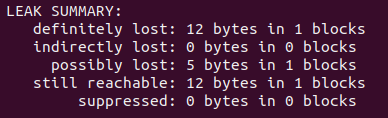
\includegraphics[width=0.7\textwidth]{leakResume.png}
%  \caption{Rezime curenja memorije}
%  \label{fig:slika2.13}
%\end{figure}

\begin{lstlisting}[style=terminal,caption={Rezime curenja memorije}, label={lst:slika2.13},language={bash}] 
LEAK SUMMARY: 
     definitely lost: 12 bytes in 1 blocks 
     indirectly lost: 0 bytes in 0 blocks
     possibly lost:  5 bytes in 1 blocks 
     still reachable: 12 bytes in 1 blocks
     suppressed: 0 bytes in 0 blocks
\end{lstlisting}

Ako je uključena opcija \texttt{--leak-check = full}, \textit{Memcheck} će dati detaljan izveštaj za svaki definitivno izgubljeni ili moguće izgubljeni blok, uključujući i mesto gde je alociran. Međutim, \textit{Memcheck} ne može reći kada, kako ili zašto se izgubio pokazivač na iscureli blok. Generalno, treba težiti tome da programi nemaju definitivno izgubljene ili moguće izgubljene blokove na izlazu.

Opcija \texttt{--show-leak-kind = <set>} kontroliše skup vrsta curenja koje će se prikazati kada je uključena opcija \texttt{--leak-check = full}. Inače, podrazumevana vrednost opcije \texttt{–leak-check} je \texttt{summary}.

\texttt{<set>} se definiše na jedan od sledećih načina:
\begin{enumerate}
\item Lista opcija odvojenih zarezom. Moguće opcije su: \texttt{definite, indirect, possible, reachable}.
\item \texttt{All} - za specifikaciju svih vrsta curenja.
\item \texttt{None} -  za prazan skup.
\end{enumerate}
Podrazumevana vrednost za vrste curenja koje se prikazuju je \texttt{--show-leak-kinds = definite, possible}.

Na listingu \ref{lst:slika2.14} prikazan je izveštaj koji daje \textit{Memcheck} o definitivnom gubitku bloka veličine 12 bajta, još uvek dostupnom bloku veličine 12 bajta, moguće izgubljenom bloku veličine 5 bajta, kao i liniju u programu gde su oni alocirani. 
%\begin{figure}[!ht]
%  \centering
%  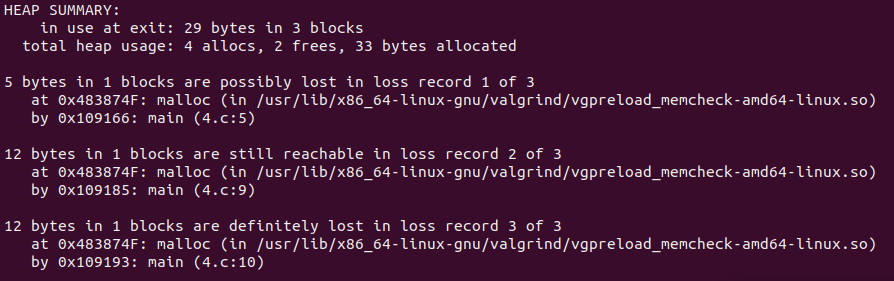
\includegraphics[width=0.7\textwidth]{heapResume.png}
%  \caption{Izveštaj o curenju memorije}
%  \label{fig:slika2.14}
%\end{figure}

\begin{lstlisting}[style=terminal,caption={Izveštaj o curenju memorije}, label={lst:slika2.14},language={bash}] 
HEAP SUMMARY:
    in use at exit: 29 bytes in 3 blocks
   total heap usage: 4 allocs, 2 frees, 33 bytes allocated
   
5 bytes in 1 blocks are possibly lost in loss record 1 of 3
    at Ox483874F: malloc (in /usr/lib/x86_64-linux-gnu/valgrind/vgpreload_memcheck-amd64-linux.so)
    by 0x109166: main (4.c:5)

12 bytes in 1 blocks are still reachable in loss record 2 of 3
    at Ox483874F: malloc (in /usr/lib/x86_64-linux-gnu/valgrind/vgpreload_memcheck-amd64-linux.so)
    by 0x109185: main (4.c:9)

12 bytes in 1 blocks are definitely lost in loss record 3 of 3
    at Ox483874F: malloc (in /usr/lib/x86_64-linux-gnu/valgrind/vgpreload_memcheck-amd64-linux.so)
    by 0x109193: main (4.c:10)
\end{lstlisting}

\textit{Memcheck} koristi odgovarajući kriterijum za prijavljivanje i tretman grešaka vezanih za curenje memorije, budući da postoje različite vrste curenja memorije različitih težina. Ukoliko je uključena opcija \texttt{--leak-check=full}, \textit{Memcheck} će smatrati da je curenje memorije greška, odnosno, ukoliko podaci o curenju memorije nisu prikazani, iako oni postoje, \textit{Memcheck} smatra da to curenje nije greška. Takođe, definitivno i moguće izgubljene blokove \textit{Memcheck} smatra greškom, dok indirektno izgubljene i još uvek dostupne blokove ne smatra greškom \cite{Memcheck}.

\begin{itemize}
\item[$\textendash$] Ako podaci o curenju memorije nisu prikazani, smatra se da to curenje nije ,,greška''.
\item[$\textendash$] Definitivno i moguće izgubljeni blokovi se smatraju za pravu ,,grešku'', dok indirektno izgubljeni i još uvek dospuni blokovi se ne smatraju kao greška \cite{ValgrindDOC}. 
\end{itemize}

\section{Ostali važni alati Valgrind distribucije}

U ovoj sekciji biće obrađeni ostali važni alati \textit{Valgrind} distribucije. Biće reči o njihovoj osnovnoj nameni i načinu korišćenja. 

Da bi uspešno izvršili analizu alatima \textit{Cashegrind}, \textit{Callgrind} i \textit{DHAT} neophodno je kompajlirati program sa opcijom za debug mod (opcija \texttt{-g}) i uključenom optimizacijom, jer nema smisla profajlirati k\^od koji je drugačiji od onoga koji će se normalno izvršavati. Za analizu programa alatom \textit{Massif} neophodno je kompaljirati program sa opcijom \texttt{-g}, dok nivo optimizacije nije od presudnog značaja. Što se alata \textit{Helgrind} i \textit{DRD} tiče, oni nisu zavisni od uslova kompilacije, tj.~opcije \texttt{-g} i uključene optimizacije.

\subsection{Cachegrind}
\textit{Cachegrind} je alat koji simulira i prati kako program pristupa keš memoriji \cite{Cachegrind}. Takođe, može se koristiti i za profajliranje izvršavanja grana. Simulira mašinu sa nezavisnim kešom instrukcija prvog nivoa i kešom podataka (I1 i D1), potpomognutim objedinjenom keš memorijom drugog nivoa (L2). 

Što se modernih mašina tiče, tj. onih mašina sa tri ili četiri nivoa keš memorije, u slučajevima kada \textit{Cachegrind} može automatski otkriti konfiguraciju keš memorije, \textit{Cachegrind} simulira pristup kešu prvog i poslednjeg nivoa, tj.~\textit{Cachegrind} simulira \textit{I1, D1 i LL}. Ovakav pristup posledica je toga što keš memorija poslednjeg nivoa (\textit{LL}) ima najveći uticaj na vreme izvršavanja, jer maskira pristupe glavnoj memoriji. Dalje, \textit{L1} keš memorije često imaju malu asocijativnost, pa se njihovom simulacijom mogu otkriti slučajevi kada k\^od loše interaguje sa ovom keš memorijom \cite{Cachegrind}.

Da bi se koristio alat \textit{Cachegrind} neophodno je podesiti opciju \texttt{–tool=cachegrind}. Izvršavanje programa će trajati dugo, a po završetku štampaće se sažeti statistički podaci. Pored štampanja sažetka na standardni izlaz, \textit{Cachegrind} u odgovarajuću datoteku upisuje i detaljnije informacije o profajliranju. Za dobijanje detaljnijih informacija koristimo pomenutu datoteku kao ulaz za \texttt{cg\_annotate}, koji je deo paketa \textit{Valgrind}. Alternativno, možete koristiti \texttt{cg\_diff} za razlikovanje više izlaza iz alata \textit{Cachegrind}, koje kasnije koristimo kao ulaz za \texttt{cg\_annotate} \cite{Cachegrind}.

\subsection{Callgrind}

\textit{Callgrind} je alat za profajliranje koji generiše istoriju poziva funkcija korisničkog programa u vidu grafa. Prikupljeni podaci podrazumevano se sastoje od broja izvršenih instrukcija, njihovog odnosa sa linijama izvršnog koda, odnosa pozivaoc/pozvan između funkcija, kao i broja takvih poziva. Opciono, simulacija keš memorije i/ili profajliranje grana (slično \textit{Cachegrind}-u) mogu dati dodatne informacije o ponašanju aplikacije u toku izvršavanja \cite{Callgrind}. Alat sadrži neka preklapanja sa \textit{Cachegrind} - om, ali takođe pruža neke informacije koje \textit{Cachegrind} ne pruža.

Da bi se koristio \textit{Callgrind}, potrebno je navesti opciju komandne linije \texttt{--tool = callgrind} u komandnoj liniji \textit{Valgrind}-a. Nakon završetka programa i rada alata, generiše se odgovarajuća datoteka sa podacima o izvršenom profajliranju. Za prezentaciju podataka i interaktivnu kontrolu profajliranja na osnovu date datoteke, obezbeđena su dva alata komandne linije. Jedan je \texttt{callgrind\_annotate}, koji čita generisani fajl i ispisuje sortirane liste funkcija, opciono sa anotacijom izvora. Drugi je \texttt{callgrind\_control} koji omogućava interaktivno posmatranje i kontrolisanje statusa programa koji se trenutno izvršava pod kontrolom \textit{Callgrind}-a, bez zaustavljanja programa. Mogu se dobiti statistički podaci kao npr.~stanje steka, a u svakom trenutku se takođe može generisati i profil \cite{Callgrind}. 

\subsection{Helgrind}

\textit{Helgrind} je \textit{Valgrind}-ov alat za otkrivanje grešaka sinhronizacije u programima C, C++ i Fortran prilikom upotreba modela niti \textit{POSIX} \cite{Helgrind}. Model niti \textit{POSIX} prate određene apstrakcije --- skup niti koji dele zajednički adresni prostor, formiranje niti, spajanje niti, izlaz iz funkcije niti, muteksi (katanci), uslovne promenljive (obaveštenja o događajima među nitima), čitaj-piši zaključavanje, spinlokovi, semafori i barijere \cite{Helgrind}. 

Da bi se koristio ovaj alat, potrebno je navesti opciju komandne linije \texttt{--tool = helgrind} u komandnoj liniji \textit{Valgrind}-a.

\textit{Helgrind} može otkriti sledeća tri tipa grešaka:
\begin{enumerate}
\item Pogrešna upotreba interfejsa za programiranje \textit{POSIX} niti.
\item Potencijalno blokiranje prouzrokovano redosledom zaključavanja.
\item Trka sa podacima (eng. \textit{data race})  - pristup memoriji bez odgovarajućeg zaključavanja ili sinhronizacije.
\end{enumerate}

Problemi poput ovih često rezultiraju ponovljivim padovima, vremenski zavisnim padovima, mrtvim tačkama i drugim nepravilnim ponašanjem, a koji se teško mogu pronaći drugim sredstvima.

Što se pogrešne upotrebe interfejsa za programiranje \textit{POSIX} niti tiče, \textit{Helgrind} presreće pozive ka funkcijama biblioteke \textit{pthread}, i zbog toga je u mogućnosti da otkrije veliki broj grešaka. Neke od njih su: 
\begin{itemize}
\item Greške u otključavanju muteksa – slučaj nevažećeg muteksa, nezaključanog muteksa, ili muteksa zaključanog od strane druge niti.
\item Greške u radu sa zaključanim muteksom – uništavanje nevažećeg ili zaključanog muteksa, rekurzivno zaključavanje nerekurzivnog muteksa, oslobađanje memorije koja sadrži zaključan muteks \cite{Helgrind}.
\end{itemize}

Što se potencijalnog blokiranja prouzrokovanog redosledom zaključavanja tiče, \textit{Helgrind} nadgleda redosled kojim niti zaključavaju promenljive. To mu omogućava detektovanje potencijalnih zastoja koji bi mogli nastati formiranjem ciklusa zaključavanja. Na ovaj način je moguće detektovati greške koje se nisu javile tokom samog procesa testiranja programa, već se mogu javiti prilikom nekog drugog pokretanja programa \cite{Helgrind}.

Što se trke sa podacima tiče, \textit{Helgrind}-ov algoritam je (konceptualno) vrlo jednostavan - nadgleda sve pristupe memorijskim lokacijama. Ako lokaciji pristupaju dve različite niti, \textit{Helgrind} proverava da li su dva pristupa uređena relacijom ,,dogodilo se pre'' (eng. \textit{happens-before relation}). Ako je tako, to je u redu, ali ukoliko nije, \textit{Helgrind} prijavljuje trku sa podacima.

\subsection{DRD}
\textit{DRD} je \textit{Valgrind}-ov alat za otkrivanje grešaka u višenitnim programima napisanim u programskim jezicima C i C++ \cite{Drd}. Alat radi za bilo koji program koji koristi niti bazirane na modelu \textit{POSIX} \cite{Drd}. Sličan je \textit{Helgrind}-u, ali koristi različite tehnike analize i tako može naći različite probleme.

Da bi se koristio ovaj alat, potrebno je navesti opciju komandne linije \texttt{--tool = drd} u komandnoj liniji \textit{Valgrind}-a.

U zavisnosti od toga koja se višenitna paradigma koristi u programu, može se pojaviti jedna ili više grešaka:
\begin{itemize}
\item Trka sa podacima.
\item Zadržavanje katanaca - jedna nit blokira napredovanje jedne ili više drugih niti držeći predugo katanac zaključanim.
\item Pogrešna upotreba interfejsa za programiranje \textit{POSIX} niti.
\item Potencijalno blokiranje prouzrokovano redosledom zaključavanja.
\item Lažno deljenje - ako niti koje rade na različitim procesorskim jezgrima često pristupaju različitim promenljivim smeštenim u istoj liniji keš memorije, to će usporiti uključene niti zbog česte razmene linija keš memorije.
\end{itemize} 

Što se tiče grešaka vezanih za pogrešnu upotrebu interfejsa za programiranje \textit{POSIX} niti, kao i trke sa podacima, greške koje \textit{DRD} otkriva su veoma slične onim koje otkriva \textit{Helgrind}, a koje su opisane u sekciji o \textit{Helgrind}-u, uz određene minimalne razlike. Kada je u pitanju greška vezana za trku sa podacima, \textit{DRD} ispisuje poruku svaki put kada otkrije da je došlo do trke podataka \cite{Drd}. Alat \textit{DRD} svakoj niti dodeljije jedinstveni ID broj. Brojevi koji se dodeljuju nitima u svojstvu identifikatora počinju od jedinice i dodeljuju se jednokratno, odnosno jednom iskorišćeni broj ne može se više koristiti. Segment uvek započinje i završava se operacijom sinhronizacije, a sam termin se odnosi na uzastopni niz operacija učitavanja, skladištenja i sinhronizacije - sve izvršene u istoj niti. Da bi detektovao grešku trke sa podacima, \textit{DRD} analizu vrši između segmenata, što kao rezultat daje bolje performanse \cite{Drd}.

Niti moraju biti u stanju da napreduju, a da ih druge niti predugo ne blokiraju. Ponekad nit mora da sačeka dok muteks ili objekat sinhronizacije ne otključa druga nit. Pojava u kojoj jedna nit ne može da nastavi sa radom zbog blokiranja drugih niti naziva se zadržavanje katanaca (eng. \textit{lock contention})  \cite{Drd}. Ovakva pojava je nepoželjna u višenitnim sistemima, a u njenom otklanjanju pomaže alat \textit{DRD} koji otkriva ovaj tip problema. 

\subsection{Massif}

\textit{Massif} je alat za profajliranje hipa. Meri koliko memorije hipa program koristi, i na koji način. To uključuje memoriju kojoj korisnik može pristupiti, kao i memoriju koja se koristi za dodatne koncepte, poput \textit{book-keeping} bajtova i prostora za poravnanje \cite{Massif}. Takođe može izmeriti veličinu steka  programa, s tim da to ne radi podrazumevano. Profajliranje hipa može pomoći u smanjivanju količine memorije koju program koristi. Na modernim mašinama ovo pruža prednosti u vidu ubrzanja programa i smanjenja šansi za izgladnjivanje prostora za razmenu mašine (eng. \textit{swap space}) \cite{Massif}.

Može se desiti da postoji pokazivač na memoriju, ali da se ta memorija ne koristi, što je jedan vid curenja memorije. Programi koji imaju ovakvo curenje mogu s vremenom nepotrebno povećati količinu memorije koju koriste. \textit{Massif} može pomoći u identifikovanju ovakvog tipa curenja memorije \cite{Massif}.

Da bi se koristio ovaj alat, potrebno je navesti opciju komandne linije \texttt{--tool = massif} u komandnoj liniji \textit{Valgrind}-a. Nakon završetka procesa profajliranja, podaci se smeštaju u odgovarajuću datoteku. Nakon toga treba pokrenuti \texttt{ms\_print} da bi podatke iz datoteke predstavili na čitljiv način. 

\subsection{DHAT}

\textit{DHAT} je alat za ispitivanje kako programi koriste alociranu memoriju na hipu. Prati dodeljene blokove i pregleda svaki pristup memoriji da bi pronašao kom bloku, ako takav blok postoji, se pristupa. Na osnovu tačke dodeljivanja predstavlja informacije o tim blokovima, kao što su veličina, životni vek, broj čitanja i pisanja i obrasce čitanja i pisanja \cite{DHAT}. Korišćenjem ovih informacija moguće je identifikovati mesta alokacije sa sledećim karakteristikama:
\begin{itemize}
\item Potencijalna curenja tokom životnog veka procesa: blokovi koji se dodeljuju se samo akumuliraju i oslobađaju se tek na kraju izvršavanja.
\item Prekomerni promet: tačke koje zauzmu veliki deo hipa, čak i ako ga ne zadržavaju jako dugo.
\item Prekomerno prolazne: tačke koje dodeljuju vrlo kratkotrajne blokove.
\item Beskorisne ili nedovoljno iskorišćene alokacije: blokovi koji su dodeljeni, ali nisu u potpunosti popunjeni, ili su popunjeni, ali se iz njih naknadno nije čitalo.
\item Blokovi sa neefikasnim rasporedom --- segmenti kojima se nikada nije pristupilo ili sa poljima raštrkanim po bloku.
\end{itemize}

Da bi se koristio alat \textit{ DHAT} potrebno je navesti opciju komandne linije \texttt{–tool=dhat} u komandnoj liniji \textit{Valgrind}-a. Analiza programa alatom \textit{DHAT} će se izvršavati prilično sporo, a po završetku, štampaće se sažeti statistički podaci. Korisnije informacije mogu se videti sa \textit{DHAT}-ovim prikazivačem. To omogućava činjenica da pored štampanja rezimea, \textit{DHAT} u datoteku upisuje i detaljnije informacije o profajliranju. Ova datoteka je u JSON formatu i namenjena je pregledu \textit{DHAT}-ovog pregledača \cite{DHAT}. 

\subsection{BBV}

Osnovni blok je linearni presek koda sa jednom ulaznom tačkom i jednom izlaznom tačkom. Vektor osnovnog bloka (eng. \textit{basic block vector - BBV}) je lista svih osnovnih blokova unetih tokom izvršavanja programa i broj koliko je puta svaki osnovni blok pokrenut \cite{BBV}. 

\textit{BBV} je alat koji generiše osnovne blok vektore za upotrebu sa alatkom za analizu \textit{SimPoint}. \textit{SimPoint} metodologija omogućava ubrzavanje arhitektonskih simulacija pokretanjem samo malog dela programa i ekstrapolacijom ukupnog ponašanja iz ovog malog dela. Većina programa pokazuje ponašanje zasnovano na fazama, što znači da će u različito vreme tokom izvršavanja program naići na vremenske intervale u kojima se k\^od ponaša slično prethodnom intervalu. Na kraju, to znači da ako možemo da detektujemo ove intervale i grupišemo ih, približna vrednost ukupnog ponašanja programa može se dobiti samo simulacijom najmanjeg broja intervala, a zatim skaliranjem rezultata \cite{BBV}.

Da bi se kreirala datoteka osnovnog vektorskog bloka, neophodno je u komandnoj liniji \textit{Valgrind}-a navesti opciju \texttt{–tool=exp-bbv}. Nakon izvršene analize biće kreirana odgovarajuća datoteka koja sadrži vektor osnovnog bloka. Za kreiranje stvarnih \textit{SimPoint} rezultata na osnovu pređašnje generisane datoteke, potreban je uslužni program \textit{SimPoint}, dostupan na \href{http://cseweb.ucsd.edu/~calder/simpoint/}{\textit{SimPoint} veb stranici}. Uslužni program \textit{SimPoint} vrši slučajnu linearnu projekciju pomoću 15 dimenzija, a zatim k-dimenziono grupisanje kako bi izračunao koji intervali su od interesa \cite{BBV}.  

% ------------------------------------------------------------------------------
\chapter{Regularni izrazi}

U današnje vreme, programski jezici imaju veoma dobru podršku za rad sa regularnim izrazima i imaju širok dijapazon upotrebe. Jezici, a samim tim i regularni izrazi koji predstavljaju jednu klasu jezika, vrlo su važni za proces kompilacije. Kompilacija se sastoji iz nekoliko etapa, koje se kasnije dele u nekoliko faza. Jezici imaju važnu ulogu u etapi analize izvornog koda. Preduslov za ispitivanje izvornog koda jeste precizna definicija jezika \cite{Vitas}.

\section{Kratak pregled teorije jezika i regularnih izraza} 

Definicija izvornog jezika mora sadržati konačan skup simbola koje možemo koristiti u jeziku, tj.~azbuku jezika. Takođe, mora sadržati sintaksička i semantička pravila jezika, tj.~opis svih reči koje pripadaju datom jeziku kao i njihovo značenje \cite{Vitas}.

Neka je $\Sigma$ konačan skup. Reč (eng. \textit{word}) nad $\Sigma$ je svaki konačan niz $$x = (a_1, a_2, …, a_n),$$ gde je $n \geq 0$, a $a_i \in \Sigma$ za svako $\textit{i} \in [1,n]$. Broj $n$ se naziva dužina reči i obeležava se sa $|x|$. Prazna reč  obeležava se simbolom $\varepsilon$, odnosno važi $| \varepsilon |=0$. Ako je $$y = (b_1, b_2, …, b_m)$$ neka druga reč nad $\Sigma$, tada je proizvod dopisivanja, tj.~konkatenacije reči $x$ i $y$ reč $$xy =(a_1, a_2, …, a_n, b_1, b_2, …, b_m).$$
Elemente skupa $\Sigma$ nazivamo slova ili simboli, dok sam skup nazivamo alfabet ili azbuka \cite{Vitas}.

Klinijevo zatvorenje azbuke $\Sigma$, u oznaci $\Sigma^*$, je skup svih niski nad azbukom $\Sigma$. Na primer, ukoliko je $\Sigma = \{a,b\}$, onda je $$\Sigma^* = { \varepsilon, a, b, aa, ab, ba, bb, …}.$$
Neutral u odnosu na dopisivanje je prazna reč, tj.~za $\forall x\in \Sigma, x\varepsilon = \varepsilon x = x$. Skup svih reči bez prazne reči označava se kao $\Sigma^+$, tj.~$\Sigma^+ = \Sigma^* - { \varepsilon }$ \cite{Vitas}. 

\begin{defn}
Bilo koji podskup skupa $\Sigma^*$: $L \subset \Sigma^*$ predstavlja jedan (formalni) jezik nad azbukom $\Sigma$. Ako $x \in L$, onda $x$ predstavlja rečenicu jezika $L$.
\end{defn}

Neka je data azbuka $\Sigma = \{ a, b, c\}$. Neki od jezika nad ovom azbukom predstavljeni su sledećim skupovima:
\begin{itemize}
\item[] $L_1 = \{a^n | n > 0\}$ – jezik koji se sastoji od niski u kojima se proizvoljan broj puta pojavljuje simbol $a$.
\item[] $L_2 = \{a^nb^m | m, n > 0\}$ – jezik koji se sastoji od niski u kojima se proizvoljan broj puta pojavljuje simbol $a$, iza čega sledi pojavljivanje simbola $b$ proizvoljan broj puta.
\item[] $L_3 = \{ca^ncccb^m | m, n > 0\}$ – jezik koji se sastoji od niski u kojima se nakon simbola $c$ proizvoljan broj puta pojavljuje simbol $a$, iza čega sledi tri pojavljivanja simbola $c$ i pojavljivanje simbola $b$ proizvoljan broj puta.
\end{itemize}

%Nad jezicima se mogu izvršiti skupovne operacije kao što su unija, presek i razlika, kao i operacija proizvoda, kako su i sami jezici skupovi \cite{Vitas}. Pored pomenutih, nad jezicima definišemo još i operaciju proizvoda, $n$-tog stepena i zatvorenja jezika $L$.
%\begin{defn}
%Proizvod jezika $L_1$ i $L_2$ nad azbukom $\Sigma$ u oznaci $L_1L_2$ je jezik $$L_1L_2 = \{xy | x \in L_1, y \in L_2\}.$$
%Proizvod jezika je asocijativna operacija, a {$\varepsilon$} je njen neutralni element.
%\end{defn}

%\begin{defn}
%Za jezik $L$, $n$-ti stepen jezika $L$ je jezik: 
%$$L_0 = \{ \varepsilon\} $$ 
%$$L_1 = L$$
%$$L_n = LL_(n-1), za n>1.$$
%\end{defn}

%\begin{defn}
%Iteracija ili (Klinijevo) zatvorenje jezika $L$, u oznaci $L^*$, je jezik:
%$$ L^* = \bigcup_{n\geq0}L^n.$$
%Pozitivno zatvorenje jezika $L$, u oznaci $L^+$, je jezik:
%$$ L^+ = \bigcup_{n\geq1}L^n = L^* - \{\varepsilon\}.$$
%\end{defn}

\begin{defn}
Regularni izrazi nad azbukom $\Sigma$ opisuju se rekurzivno na sledeći način:
\begin{enumerate}
\item Prazan skup je regularni izraz koji se prikazuje simpolom $\emptyset$;
\item Regularni izraz $\varepsilon$ predstavlja jezik $\{\varepsilon\}$;
\item Ako je $a \in \Sigma$, onda regularni izraz $a$ predstavlja jezik $\{a\}$;
\item Ako su $p$ i $q$ regularni izrazi jezika $L(p)$ i $L(q)$, onda je:
\begin{itemize}
\item $(p+q)$ regularni izraz koji predstavlja jezik $L(p) \cup L(q)$.
\item $(pq)$ regularni izraz koji predstavlja jezik $L(p)L(q)$.
\item $(p)^*$ regularni izraz koji predstavlja jezik $(L(p))^*$.
\item $(p)$ regularni izraz koji predstavlja jezik $L(p)$.
\end{itemize}
\end{enumerate}
\end{defn}

Opisani jezik se neće promeniti ako se zagrade izostave iz regularnog izraza \cite{Vitas}. Kada prioritet operacija nije eksplicitno naveden, primenjuju se podrazumevani prioriteti nad operatorima regularnih izraza, tj.~jezika, u sledećem redosledu:
\begin{enumerate}
	\item operator $*$
	\item konkatenacija
	\item operator $+$
\end{enumerate}

\begin{defn}
Ukoliko se jezik može predstaviti regularnim izrazom, takav jezik se smatra regularnim.
\end{defn}

Važnost ove notacije ogleda se u tome što se na isti način zapisuju simbol azbuke, reč koja se sastoji od tog simbola, regularni izraz koji predstavlja taj simbol, i na kraju jezik predstavljen tim regularnim izrazom \cite{Vitas}. Kažemo da je za neki regularni izraz $p$, jezik $L(p)$ jezik opisan regularnim izrazom $p$.

Zapisivanje regularnih izraza može se znatno pojednostaviti uvođenjem sledećih konvencija:
\begin{itemize}
\item Neka je $r$ regularni izraz koji opisuje jezik $L(r)$. Jezik $(L(r))(L(r))^*$ se opisuje regularnim izrazom $(r)^+$ , dok se jezik $L(r) \cup \{\varepsilon\}$ opisuje regularnim izrazom $(r)?$;
\item Ako su $c_1, c_2, …, c_n$ karakteri, tada se regularni izraz $c_1 + c_2 + … + c_n$ može obeležiti sa $[c_1, c_2, …, c_n]$. Izraz $[c_1-c_2]$ označava sekvencu svih karaktera $c$ tdj. $c_1 \leq c \leq c_2$.
\end{itemize}

Tako na primer slova engleske abecede označavamo sa $[A-Za-z]$, dok cifre označavamo sa $[0-9]$.
 
\section{Modul re}

Alat koji ovaj rad prati razvijen je u programskom jeziku Python, a \textit{re} je modul koji pruža podršku za rad sa regularnim izrazima u Python programima. Ovaj modul pruža operacije podudaranja regularnih izraza. Važno je napomenuti da je većina operacija sa regularnim izrazima dostupna u vidu funkcija i metoda na nivou modula sa kompajliranim regularnim izrazima. Funkcije su prečice koje ne zahtevaju da prvo kompajlirate objekat regularnog izraza, ali je mana što im nedostaju neki parametri za fino podešavanje. 

Regularni izraz navodi niz karaktera koji mu odgovara, dok vam funkcije u ovom modulu omogućavaju da proverite da li se određeni niz karaktera poklapa sa datim regularnim izrazom (ili da li se regularni izraz podudara sa određenim nizom karaktera, što se svodi na istu stvar).
Neke od funkcija koje ovaj modul pruža, a koje su iskorišćene u alatu koji ovaj rad prati su sledeće:

\begin{itemize}
\item[$\textendash$]  \textit{re.search(pattern, string, flags=0)} - Skenira kroz \textit{string} tražeći prvu lokaciju na kojoj obrazac regularnog izraza daje podudaranje i vraća odgovarajući objekt podudaranja. Vratiće \textit{None} ako nijedna pozicija u nizu karaktera ne odgovara obrascu.
\item[$\textendash$]  \textit{re.match(pattern, string, flags=0)} - Ako se nula ili više znakova na početku niza karaktera \textit{string}  podudaraju sa regularnim izrazom, vratiće odgovarajući objekt podudaranja. Vratiće \textit{None} ako se niz ne podudara sa obrascem.
\item[$\textendash$]  \textit{re.split(pattern, string, maxsplit=0, flags=0)} - Podeliće nisku \textit{string} pojavljivanjima koja se poklapalu sa \textit{pattern}. 
\item[$\textendash$]  \textit{re.findall(pattern, string, flags=0)} - Vraća sva podudaranja \textit{pattern}-a u \textit{string}-u kao listu stringova, tj.~niski. Niska u kojoj se traže preklapanja - \textit{string}, skenira se s leva na desno, a poklapanja se vraćaju u redosledu u kom se i javljaju. 
\item[$\textendash$]  \textit{re.sub(pattern, repl, string, count=0, flags=0)} - Vraća string dobijen zamenom krajnjeg levog poklapanja sa \textit{pattern}-om u \textit{string}-u sa \textit{repl}. Ako poklapanje nije pronađeno, \textit{string} se vraća nepromenjen. Argument \textit{repl} može biti niz ili funkcija.
\end{itemize}

Kompajlirani objekti regularnog izraza podržavaju slične metode i atribute, s tim da je pozivanje istih u formi
\begin{center}
\texttt{pattern.funkcija(argumenti).}
\end{center}

Objekti podudaranja uvek imaju logičku vrednost \textit{True}. Budući da \textit{match()} i \textit{search()} vraćaju \textit{None} kada nema podudaranja, možete testirati da li je postojalo podudaranje jednostavnim \textit{if} izrazom. 

Objekti podudaranja podržavaju mnoge metode i atribute, a najiskorišćenija u alatu koji je razvijen, a u cilju izvlačenja potrebnih informacija iz poklapanja sa regularnim izrazom je:
\begin{itemize}
\item[$\textendash$]  \textit{Match.group([group1, ...])} - Vraća jednu ili više podgrupa podudaranja. Ako postoji jedan argument, rezultat je jedan string, dok ako postoji više argumenata, rezultat je t-orka sa jednom stavkom po argumentu. Bez argumenata, \textit{group1} je  podrazumevano nula, tj.~vraća se ceo \textit{Match} objekat. Ako je indeks \textit{group} u opsegu [1,99], to je string koji odgovara odgovarajućoj grupi u zagradama na toj poziciji. Ako je broj grupe negativan ili veći od broja grupa definisanih u obrascu, biće izbačen izuzetak \textit{IndexError}. Ako je grupa sadržana u delu uzorka koji se ne podudara, odgovarajući rezultat je \textit{None}. Ako je grupa sadržana u delu uzorka koji se podudarao više puta, vraća se poslednje podudaranje \cite{reModule}.
\end{itemize}

Primer korišćenja funkcije \textit{group} dat je na listingu \ref{lst:slika3.1}.
%\begin{figure}[!ht]
%  \centering
%  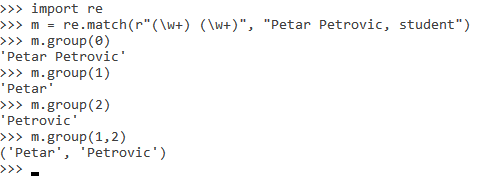
\includegraphics[width=0.7\textwidth]{reModule.png}
%  \caption{Primer korišćenja funkcije \textit{group} modula \textit{re}}
%  \label{fig:slika3.1}
%\end{figure}

\begin{lstlisting}[style=terminal,caption={Primer korišćenja funkcije \textit{group} modula \textit{re}}, label={lst:slika3.1},language={bash}] 
>>> import re
>>> m = re.match(r"(\w+) (\w+)", "Petar Petrovic, student")
>>> m.group(0)
'Petar Petrovic'
>>> m.group(1)
'Petar'
>>> m.group(2)
'Petrovic'
>>> m.group(1,2)
('Petar', 'Petrovic')
>>>
\end{lstlisting}

% ------------------------------------------------------------------------------

% ------------------------------------------------------------------------------
\chapter{Alat Koronka}
Alat \textit{Koronka} predstavlja alat koji automatski otkriva greške u kodu napisanom u programskom jeziku C koristeći alat \textit{Memcheck}, a zatim ih ispravlja ukoliko je to u njegovoj moći. Alat je razvijan pod \textit{Linux} okruženjem, a implementiran u programskom jeziku \textit{Python}. Alat je nazvan \textit{Koronka}, zbog situacije u kojoj se ceo svet našao početkom 2020. godine. Osnovna svrha alata je demonstracija rada alata \textit{Valgrind}, kao i tumačenje izveštaja o greškama koje \textit{Valgrind} daje i njihovo uspešno otklanjanje. Alat je slobodno dostupan i nalazi se na linku \url{https://github.com/LMladenovic/Error_fixing_tool}. Na pomenutom linku se nalaze neophodne datoteke alata, opis sistema, kao i skup test primera i njihova pokretanja.

\section{Korišćenje alata}
Da biste pokrenuli alat \textit{Koronka} neophodno je da prethodno instalirate \textit{GCC} kompajler, sam alat \textit{Valgrind}, kao i \textit{Python}. U razvoju alata korišćen je \textit{Python2.7}, pa su mogući neki neželjeni efekti prilikom pokretanja na novijim verzijama. Alat se pokreće sledećom komandom:
\begin{center}
\texttt{python koronka.py [files=[list of files]] [structures=[list of user defined structures]] path to c file [other arguments]}
\end{center}
Navedeni arumenti podrazumevaju sledeće:
\begin{itemize}
\item \texttt{files} - sadrži dodatne fajlove glavnog programa (navedenog u okviru \textit{path to c file}) koji se analizira (npr. \textit{.h} fajlove). Ukoliko se program sastoji iz više fajlova, neophodno je da se navedu kao argument. Ako se ne navede argument \textit{files}, niz \textit{files} će sadržati samo glavni program (\textit{c file}) i biće u mogućnosti da vrši promene samo nad njim.
\item \texttt{structures} - predstavlja korisnički definisane strukture u okviru programa. Kako alat podrazumevano radi samo sa primitivnim tipovima podataka, ukoliko u programu postoje korisnički definisane strukture, a ne navedu se kao argument, \textit{Koronka} neće biti u mogućnosti da ispravi greške povezane sa tim strukturama, naravno, ukoliko postoje.
\item \texttt{other args} - argumenti programa koji se analizira.
\end{itemize}

Takođe, alat \textit{Koronka} sadrži i opciju \texttt{--help } čijim će navođenjem biti ispisano uputstvo za upotrebu alata. 

Sve argumente koji se navedu prilikom pokretanja alata \textit{Koronka} obradiće funkcija za obrađivanje argumenata komandne linije. Nakon pokretanja alata, u direktorijumu alata će se kreirati direktorijum u formatu \textit{datum pokretanja-vreme pokretanja}. U njega će se kopirati svi podaci navedeni kao arugment \textit{files}, kao i glavni program nad kojim se vrši analiza i nad njima će biti vršene odgovarajuće promene u skladu sa otkrivenim greškama. Originalni fajlovi ostaće nepromenjeni. Po završetku rada alata, u pomenutom direktorijumu će se naći još dva fajla. Prvi je \textit{ExecutionReport} koji sadrži detaljan izveštaj o radu alata, koje greške je našao, na koji način ih je rešio, koje fajlove, odnosno linije koda u njima je izmenio. Drugi, pod nazivom \textit{ValgrindLOG.txt}, predstavlja izlaz alata \textit{Valgrind}, koji će se u procesu rada alata koristiti za parsiranje grešaka koje nađe alat \textit{Memcheck}. Ukoliko se analizira ispravljeni program nakon završetka rada alata alatom \textit{Memcheck}, biće dobijen isti izlaz koji možete videti u datoteci \textit{ValgrindLOG.txt}. Način i logika rada alata biće opisani u sekcijama koje slede.

\section{Algoritam izvršavanja}\label{algoritam}
Pri pokretanju alata generiše se odgovarajući direktorijum, u njega se kopiraju svi navedeni (potrebni) fajlovi, formiraju se nizovi \textit{structures}, \textit{files} i \textit{history}. Nakon početnih podešavanja sledi iterativno kompilacija programa i analiza \textit{Valgrind}-ovim alatom \textit{Memcheck} čiji izlaz se smešta u datoteku \textit{ValgrindLOG.txt}. Ovaj fajl se parsira, i iz njega se čitaju informacije o greškama iterativno. Kad alat naiđe na grešku, parsira je, nakon čega proba da je ispravi ukoliko je u mogućnosti. Ukoliko nađe rešenje koje već nije primenjeno, biće implementirano nakon čega alat ide u novu iteraciju kompilacije i provere grešaka, uz prethodno ažuriranje istorije i izveštaja o ispravljenim greškama. Proces se ponavlja dokle god ima grešaka koje nisu ispravljene, a koje je \textit{Koronka} u mogućnosti da ispravi. Grafički prikaz algoritma dat je na slici \ref{fig:slika4.4}.

\begin{figure}[!ht]
  \centering
  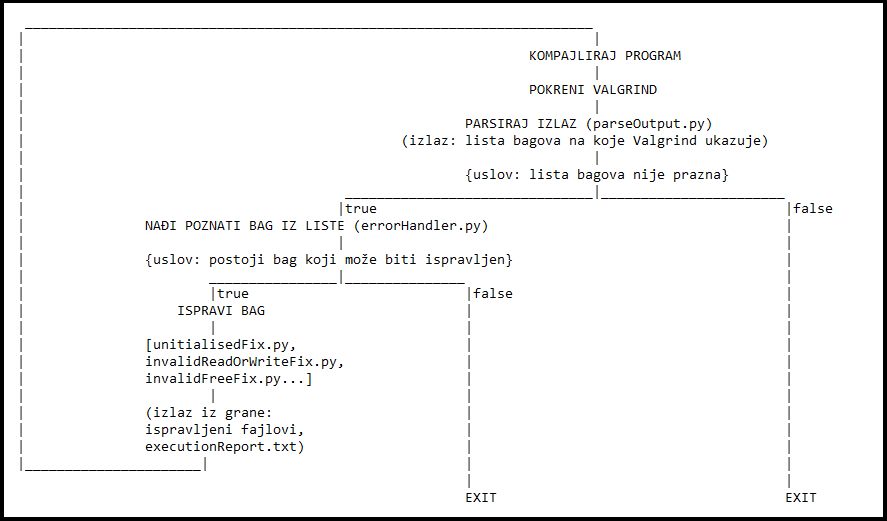
\includegraphics[width=0.9\textwidth]{ExecutingAlgorithm.png}
  \caption{Algoritam izvršavanja alata \textit{Koronka} sa pratećim fajlovima koji se koriste za njegovu realizaciju}
  \label{fig:slika4.4}
\end{figure}

\section{Klasa greške}
Prilikom ispravljanja grešaka, greška koja se trenutno obrađuje biće predstavljena kao objekat klase \textit{ErrorInfo}. Na listingu \ref{lst:slika4.1} prikazana je pomenuta klasa.

Podaci koje klasa sadrži su sledeći:
\begin{itemize}
\item \textit{errorType} - sadrži informaciju o tipu greške, npr. nevalidno oslobađanje memorije, nedozvoljeno čitanje/pisanje itd.
\item \textit{valgrindOutput} - sadrži kompletan segment teksta koji je \textit{Valgrind} ispisao za grešku koja se trenutno obrađuje za potrebe dodatnog parsiranja informacija o grešci. Primer sadržaja za jednu grešku prikazan je na slici \ref{fig:slika4.3}.
\item \textit{files} - sadrži niz fajlova koji su povezani sa greškom, a koji bi eventualno bili ispravljeni.
\item \textit{changedFile} - sadrži ime fajla koji će biti promenjen.
\item \textit{changedLine} - sadrži tačnu liniju koda u fajlu \textit{changedFile} koja će biti promenjena.
\item \textit{problemLines} - sadrži linije u kodu koje su izazvale grešku koja se ispravlja.
\item \textit{errorReason} - sadrži razlog koji je izazvao grešku, npr. upotreba neinicijalizovane vrednosti sa steka, odnosno hipa.
\item \textit{bug} - sadrži bag u kodu, tj.~sadržaj linije koda koji je izazvao grešku.
\item \textit{bugFix} - sadrži ispravku greške, tj.~sadržaj kojim treba zameniti \textit{changedLine} da bi greška bila ispravljena.
\end{itemize}

\begin{lstlisting}[style=mystyle,caption={Potpis klase \textit{ErrorInfo}}, label={lst:slika4.1},language={Python}] 
class ErrorInfo:

	# Initialisation with errorType
	def __init__(self, errorType, valgrindOutput, files):
        	self.errorType = errorType
		self.valgrindOutput = valgrindOutput
		self.files = files
		self.changedFile = ''
		self.changedLine = -1
		self.problemLines = []
		self.errorReason = []
		self.bug = ''
		self.bugFix = ''
\end{lstlisting}
%\begin{figure}[!ht]
%  \centering
%  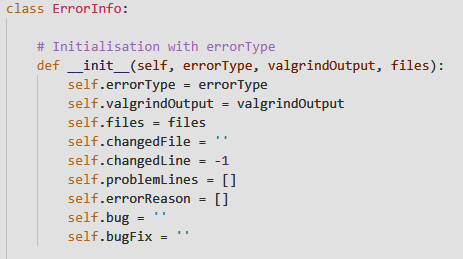
\includegraphics[width=0.7\textwidth]{ErrorClass.png}
%  \caption{Potpis klase \textit{ErrorInfo}}
%  \label{fig:slika4.1}
%\end{figure}

Za sve atribute klasa sadrži odgovarajuće metode za postavljanje i čitanje vrednosti, kao i funkciju  \textit{isKnownReason} koja proverava da li je razlog greške poslat kao argument, zaista razlog koji je izazvao grešku koja se obrađuje. Prikaz funkcije dat je na listingu \ref{lst:slika4.2}.

\begin{lstlisting}[style=mystyle,caption={Prikaz funkcije koja proverava validnost razloga greške}, label={lst:slika4.2},language={Python}] 
def isKnownReason(self, newReason):
	for reason in self.errorReason:
		if reason.find(newReason) >= 0:
			return True
			break
	return False
\end{lstlisting}

%\begin{figure}[!ht]
%  \centering
%  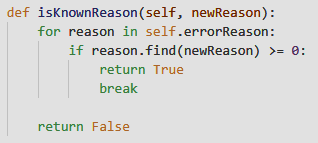
\includegraphics[width=0.7\textwidth]{ErrorReason.png}
%  \caption{Prikaz funkcije koja proverava validnost razloga greške}
%  \label{fig:slika4.2}
%\end{figure}

Na slici \ref{fig:slika4.3} prikazan je segment izveštaja alata \textit{Valgrind} koji predstavlja jednu grešku koju treba ispraviti. Žutom bojom je obeležen deo koji predstavlja tip greške, zelenom bojom deo koji predstavlja razlog greške, dok su plavom bojom obeležene sumnjive(problematične) linije. Ti podaci će redom biti smešteni u \textit{errorType}, \textit{errorReason} i \textit{problemLines}. Sve potrebne informacije od značaja iz datog segmenta izveštaja dobićemo upotrebom regularnih izraza.

\begin{figure}[!ht]
  \centering
  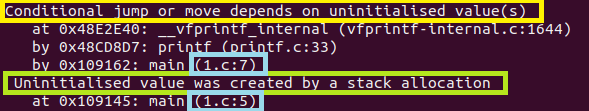
\includegraphics[width=0.9\textwidth]{ErrorClassExplaination.png}
  \caption{Prikaz izveštaja za jednu grešku}
  \label{fig:slika4.3}
\end{figure}

Na osnovu \textit{errorType} i \textit{errorReason} biće određeno koji će šablon biti upotrebljen za ispravljanje greške. Na osnovu \textit{problemLines} biće pronađena tačna linija koda koja je izazvala grešku, a iz nje izvučeni podaci koji su neophodni za ispravljanje greške, kao i iz ostalih linija ukoliko sadrže informacije od značaja. Kada se neophodni podaci o grešci izvuku i nađe njeno rešenje, biće postavljene vrednosti \textit{changedFile}, \textit{changedLine}, \textit{bug}, \textit{bugFix}. Kada se obezbede svi podaci, dalje izvršavanje alata prepušta se sistemu za praćenje istorije promena.

\section{Mehanizam praćenja istorije}\label{istorija}
Sve promene koje je alat \textit{Коronka} izvršio nad fajlovima biće praćene pomoću mehanizma za praćenje istorije. Svaka promena biće sačuvana pojedinačno u nizu \textit{history} u vidu uređene trojke \textit{(izmena u kodu, promenjena linja koda, fajl nad kojim se vrši promena)}. Ovakav vid praćenja istorije je dobar iz više razloga. Na primer, može se desiti da imamo iste naredbe koje izazivaju grešku u dva različita fajla. Promena tih naredbi bez praćenja fajla nad kojim se vrši promena ne bi bila moguća u oba fajla, ukoliko je ispravka greške opet ista naredba sa određenim dodacima. Takođe, može se desiti na primer da u istom fajlu imamo dva bloka unutar kojih postoji linija koja izaziva problem. To su dakle dve greške, čije rešenje mogu biti dve potupuno iste naredbe, izmenjene u dve različite linije koda u istom fajlu. Ukoliko mehanizam praćenja istorije ne pamti i liniju koda u kojoj su promene izvršene, to neće biti moguće.  

Prilikom pokretanja alata niz \textit{history} sadrži samo jednu trojku, tj.~\textit{(' ', -1, ' ')}. Kako se greške iterativno ispravljaju, svaka iteracija predstavlja pokušaj alata da datu grešku ispravi, što je bliže opisano u sekciji \ref{algoritam}. Za mehanizam praćenja istorije je to važno jer će on biti taj koji će validirati trenutni predlog za ispravku greške koje je alat našao. Prvi slučaj je da se predlog ispravke ne nalazi u istoriji, on će biti implementiran i dodat isoriji izmena u nadi da će se greška uspešno ispraviti. U drugom slučaju, predlog ispravke se već nalazi u istoriji izmena, što je signal alatu da je predlog rešenja već implementiran i da ta implementacija nije ispravila grešku, te da alat nastavi sa traženjem novog rešenja. U teoriji, ukoliko alat iskoristi sve mehanizme za ispravljanje određene greške koje poseduje, tj.~implementira sve predloge rešenja koje je u mogućnosti da predloži, a greška ostane neispravljena, alat će nastaviti sa radom i pokušati da ispravi ostale greške, ukoliko postoje. Navedena greška će ostati neispravljena, a korisnik će biti obavešten da postoji greška koja nažalost nije ispravljena, samim tim što će se izveštaj o njoj nalaziti u datoteci \textit{ValgrindLOG.txt}. Prilikom nalaženja rešenja koje će zaista i biti implementirano, to rešenje biva dodato u istoriju, a alat nastavlja sa iteracijama ispravljanja ostalih grešaka.

\section{Šabloni za ispravljanje grešaka}
Alat \textit{Koronka} sadrži nekoliko šablona od kojih svaki ispravlja određenu vrstu grešaka. Šablon koji će biti primenjen za ispravljanje date greške određen je vrstom greške kao i razlogom koji je datu grešku izazvao, a koje dobijamo iz izveštaja koji daje \textit{Memcheck}. Bez obzira na optimizaciju koji \textit{Memcheck} poseduje za ispisivanje izveštaja o grešci, i dalje ispisuje par paragrafa koji se odnose na istu grešku, sa različitim razlogom, odnosno tipom (pogledati npr. listing \ref{lst:slika2.7}). To je posledica principa rada alata \textit{Memcheck}, koji prati izvršavanje od početka, odnosno prati indirektan put te greške. To dalje znači da ne moramo da mapiramo sve tipove i razloge grešaka, već samo one koje će nam dati dovoljno informacija za ispravljanje greške. Nakon što se greška ispravi i program pusti na novu fazu kompilacije i analize alatom \textit{Memcheck}, izveštaj koji će se generisati neće sadržati paragrafe koje je sadržao ranije, a za čije smo ispravljanje koristili samo jedan paragraf. Ovakva implementacija doprinosi efikasnosti alata, kako smo za otklanjanje određene greške koristili samo neophodnu količinu podataka, a ne sve podatke koje smo imali. Šabloni su smešteni u fajlove sa sufiksom \textit{Fix}, dok u imenu sadrže i tip greške koji ispravljaju. 

Kao što je već rečeno, šabloni su orijentisani prvenstveno prema tipu greške koju ispravljaju, pa će njihovo izlaganje biti realizovano kroz tipove grešaka koje ispravljaju. 

\subsection{Korišćenje neinicijalizovane vrednosti}
Šablon koji ispravlja greške korišćenja neinicijalizovane vrednosti mapiran je na osnovu opisa koji daje alat \textit{Memcheck}, tj.~\textit{,,Conditional jump or move depends on uninitialised value(s)''}, dok razlozi za grešku mogu biti \textit{,,Uninitialised value was created by a stack allocation''} i \textit{''Uninitialised value was created by a heap allocation''}, u zavisnosti od toga da li je reč o statičkoj, odnosno dinamički alociranoj memoriji. Ispis alata \textit{Valgrind} koji dobijamo za ovaj tip greške u slučaju statičke memorije, a na osnovu kog je ispravljamo, dat je na listingu \ref{lst:slika4.5}.

%\begin{figure}[!ht]
%  \centering
%  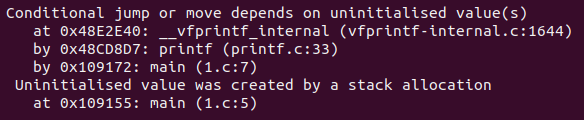
\includegraphics[width=0.9\textwidth]{UninitialisedStatic.png}
%  \caption{Ispis greške korišćenja statičke neinicijalizovane promenljive}
%  \label{fig:slika4.5}
%\end{figure}

\begin{lstlisting}[style=terminal,caption={Ispis greške korišćenja statičke neinicijalizovane promenljive}, label={lst:slika4.5},language={bash}]   
==7863==  Conditional jump or move depends on uninitialised value(s)
==7863==      at 0x48E2E40: _vfprintf_internal (vfprintf-internal.c:1644) 
==7863==      by Ox48CD8D7: printf (printf.c:33)
==7863==      by 0x109172: main (1.c:7)
==7863==  Uninitialised value was created by a stack allocation
==7863==      at 0x109155: main (1.c:5)
\end{lstlisting}

Iz datog izveštaja dobijamo informacije od važnosti za ispravljanje greške kao što su linije koda u kojima se koristi neinicijalizovana promenljiva, kao i liniju koda i fajl u kom počinje blok u kom je ta promenljiva definisana. Kako nemamo tačnu liniju koda u kojoj je promenljiva definisana, već blok, grešku ćemo ispraviti inicijalizovanjem svih neinicijalizovanih vrednosti u okviru tog bloka. 

Analizom linija koda datog bloka poklapanjem sa regularnim izrazom 
$$ ([\quad\textbackslash t]*)([a-zA-Z_-]+)[\quad]+([a-zA-Z0-9_-]+).*; $$
dobijamo liniju koda gde imamo neinicijalizovanu definisanu promenljivu. Ona može biti i višedimenziona, pa pre inicijalizacije vršimo i tu proveru da bi je, ukoliko je to slučaj, adekvatno inicijalizovali. Iz rezultata dobijenih poklapanjem sa regularnim izrazima izvlačimo podatke poput tipa promenljive, imena, a u slučaju višedimenzionog niza još i dimenzije. Na primer, primenom navedenog regularnog izraza koristeći funkciju \textit{search} modula \textit{re} nad odgovarajućom linijom koda dobijamo objekat poklapanja. Iz datog objekta, primenom funkcije \textit{group} dobijamo segmente koje odgovaraju uparenim zagradama, i to:
\begin{itemize}
\item tip promenljive na osnovu \textit{matchObject.group(2)}
\item ime promenljive na osnovu \textit{matchObject.group(3)}
\end{itemize} 
Za inicijalizaciju promenljivih koristimo funkciju prikazanu na listingu \ref{lst:slika4.6}, dok u slučaju nizova, odnosno višedimenzionih nizova, koristimo pomoćnu funkciju koja koristi petlje za inicijalizaciju, a koja se suštinski oslanja na funkciju sa listinga \ref{lst:slika4.6}.

\begin{lstlisting}[style=mystyle,caption={Funkcija inicijalizacije}, label={lst:slika4.6},language={Python}] 
def initialise(varType):
	initialisator = {
		'int': '0',
		'double': '0',
		'float': '0',
		'boolean': 'False',
		'char': '\'\\0\'',
		'short': '0',
		'long': '0'
	    }
	
	if varType in initialisator:
		return initialisator[varType]
	else:
		return 'Invalid'
\end{lstlisting}

%\begin{figure}[!ht]
%  \centering
%  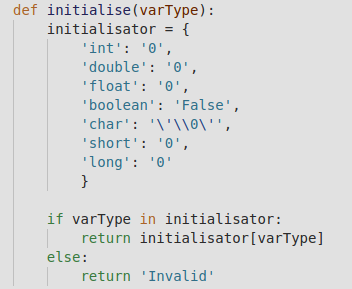
\includegraphics[width=0.5\textwidth]{InitialisationFunction.png}
%  \caption{Funkcija inicijalizacije}
%  \label{fig:slika4.6}
%\end{figure} 

U slučaju da je neinicijalizovana promenljiva korisnički definisana struktura, ukoliko je ona navedena kao argument komandne linije, alat će biti u mogućnosti da ispravi ovu grešku. Ispravljanje se sastoji u tome što će alat pronaći kako je ta struktura definisana, odnosno koji su njeni činioci. Koristeći odgovarajuću funkciju iz \textit{userDefinedStructuresHandler}-a, u kome su definisane sve operacije nad korisnčkim strukturama, inicijalizovaće celu strukturu, redom, inicijalizujući njene činioce, indirektno koristeći funkciju sa listinga \ref{lst:slika4.6}. Takođe, podržana je i inicijalizacija nizova, odnosno višedimenzionih nizova korisničkih struktura. 

Ispravku greške formiramo tako što zamenimo problematičnu liniju koda linijom gde je promenljiva definisana i inicijalizovana, dok u slučaju nizova i višedimenzionih nizova, problematičnu liniju menjamo blokom koda koji se sastoji iz definicije promenljive nakon koje sledi inicijalizacija korišćenjem petlje, odnosno petlji u slučaju višedimenzionih nizova. 

Ispis alata \textit{Valgrind} koji dobijamo za ovaj tip greške u slučaju dinamički alocirane memorije, tj.~upotrebe pokazivača, a na osnovu kog je ispravljamo, dat je na listingu \ref{lst:slika4.7}.

%\begin{figure}[!ht]
%  \centering
%  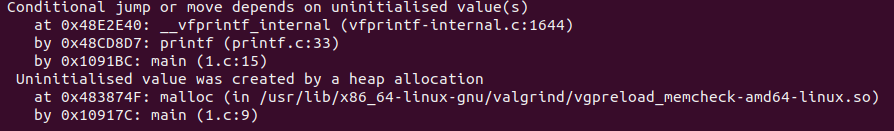
\includegraphics[width=0.9\textwidth]{UninitialisedDinamic.png}
%  \caption{Ispis greške korišćenja dinamiči alocirane neinicijalizovane promenljive (pokazivača)}
%  \label{fig:slika4.7}
%\end{figure} 

\begin{lstlisting}[style=terminal,caption={Ispis greške korišćenja dinamiči alocirane neinicijalizovane promenljive (pokazivača)}, label={lst:slika4.7},language={bash}]   
==3756==  Conditional jump or move depends on uninitialised value(s)
==3756==      at Ox48E2E40: __vfprintf_internal (vfprintf-internal.c:1644)
==3756==      by Ox48CD8D7: printf (printf.c:33)
==3756==      by Ox1091BC: main (1.c:15)
==3756==  Uninitialised value was created by a heap allocation
==3756==      at Ox483874F: malloc (in /usr/lib/x86_64-linux-gnu/valgrind/vgpreload_memcheck-amd64-linux.so) 
==3756==      by Ox10917C: main (1.c:9)
\end{lstlisting}

Za razliku od greške upotrebe neinicijalizovane promenljive koja je statički definisana, ovde, u izveštaju pored linija koda u kojima se koristi ta promenljiva dobijamo i informaciju o tačnoj liniji koda i fajlu u kom je promenljiva kreirana. Način inicijalizacije je isti kao kod statički definisanih promenljivih, dok potrebne informacije dobijamo primenom odgovarajućih regularnih izraza. Takođe, ukoliko je promenljiva samo pokazivač, bez alokacije memorije prilikom definicije iste, njena vrednost biće postavljena na \textit{NULL}. Regularni izraz koji koristimo u ovom slučaju jeste 
$$ (malloc|calloc|realloc)(.+); $$
dok se preciznije dobijanje informacije o grešci dobija specijalizacijom pomenutog izraza. Na osnovu rezultata primene pomenutih regularnih izraza dobijamo informacije o tipu pokazivača, imena pokazivača kao i veličini alocirane memorije. Primenom funkcije \textit{search} koristeći navedeni regularni izraz na osnovu \textit{matchObject.group(1)} dobijamo informaciju koja funkcija alokacije je iskorišćena. Dalje, u zavisnosti od te funkcije primenjuju se pomenuti specijalizovani regularni izrazi i odgovarajuće transformacije nad  \textit{matchObject.group(2)} u cilju dobijanja svih preostalih neophodnih informacija. Takođe, i u ovom slučaju alat poseduje podršku za rad sa korisnički definisanim strukturama. 

Nakon sakupljanja potrebnih informacija, ispravku greške formiramo na isti način kao i kod statiči definisanih promenljivih, tj.~problematičnu liniju menjamo blokom koji pored te linije sadrži i k\^od koji vrši inicijalizaciju, indirektno naslonjen na funkciju sa listinga \ref{lst:slika4.6} i inicijalizacione funkcije koje koriste petlje.

\subsection{Nevalidno čitanje/pisanje}
Šablon koji ispravlja greške nevalidnog čitanja/pisanja mapiran je na osnovu opisa koji daje alat \textit{Memcheck}, tj.~\textit{,,Invalid read of size x''} u slučaju nevalidnog čitanja, odnosno \textit{,,Invalid write of size x''} u slučaju nevalidnog pisanja, gde je \textit{x} broj bajtova. Razlog greške kojim se ova greška mapira je \textit{,,Address adr is y bytes after a block of size z alloc'd''} u slučaju prekoračenja s desne strane, odnosno \textit{,,Address adr is y bytes before a block of size z alloc'd''} u slučaju prekoračenja s leve strane, gde \textit{adr} predstavlja heksadekadni zapis adrese, a \textit{y} i \textit{z} broj bajtova. To se jasno može videti na listingu \ref{lst:slika4.8}.

%\begin{figure}[!ht]
%  \centering
%  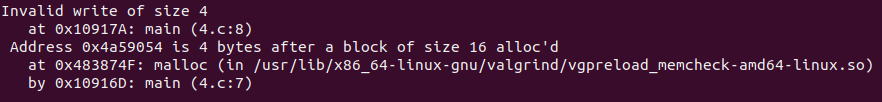
\includegraphics[width=0.9\textwidth]{InvalidReadErrorExample.png}
%  \caption{Ispis greške nevalidnog čitanja}
%  \label{fig:slika4.8}
%\end{figure} 

\begin{lstlisting}[style=terminal,caption={Ispis greške nevalidnog čitanja}, label={lst:slika4.8},language={bash}]   
==4289==  Invalid write of size 4
==4289==      at Ox10917A: main (4.c:8)
==4289==  Address 0x4a59054 is 4 bytes after a block of size 16 alloc'd
==4289==      at Ox483874F: malloc (in /usr/lib/x86_64-linux-gnu/valgrind/vgpreload_memcheck-amd64-linux.so) 
==4289==      by Ox10916D: main (4.c:7)
\end{lstlisting}

Analizom segmenta sa listinga \ref{lst:slika4.8}, odnosno samo razloga i tipa greške, možemo da dobijemo informaciju koliko je velika memorija kojoj pokušavamo da pristupimo, ili da je izmenimo, a koja nije alocirana. Moguća ispravka je adkevatno računanje izraza koji se koristi za indeksiranje, ali tu vrstu ispravke ovde nije moguće uraditi. Druga ispravka bi bila da memoriju koju program alocira, a sa kojom je pokušana interakcija, proširimo za vrednost koju dobijamo primenom pomenutih informacija. Takođe, na listingu \ref{lst:slika4.8} vidimo da dobijamo i tačnu liniju koda, odnosno fajl gde je memorija alocirana. Baš tu liniju koda menjamo ispravnom, a ispravka se sastoji u tome da pogrešnu veličinu memorije koja se alocira zamenimo ispravnom, uvećanom za broj bajtova koji dobijemo analizom greške. Na ovaj način ispravljamo greške koje su povezane sa prekoračenjem s desne strane. 

U slučaju prekoračenja s leve strane, pristupamo memoriji kojoj nam nije dozvoljeno, odnosno arument pristupa je vrednost manja od 0, kako znamo da indeksi pristupa alociranoj memoriji kreću od 0. Ovu grešku ispravljamo tako što pogrešan indeks pristupa zamenimo njegovom apsolutnom vrednošću i na taj način ispravni indeksi ostaju takvi, dok pogrešne stavljamo u interval ispravnih. U slučaju da apsolutna vrednost pomenutog indeksa izaziva grešku prekoračenja s desne strane, memorija će biti proširena, odnosno ispravljaće se greška nevalidnog čitanja/pisanja u slučaju prekoračenja s desne strane.  


\subsection{Nevalidno oslobađanje memorije}
Šablon koji ispravlja greške nevalidnog oslobađanja memorije mapiran je na osnovu opisa koji daje alat \textit{Memcheck}, tj.~\textit{,,Invalid free() / delete / delete[] / realloc()''}. Za ovaj tip greške razlog nije od presudnog značaja, tako da se mapiranje vrši samo nad opisom greške. Na listingu \ref{lst:slika4.9} prikazan je segment ispisa greške koji koristimo da bismo je ispravili. Analizom ispisa sa slike dobijamo preciznu informaciju o liniji koda, kao i o fajlu gde je izvršeno nevalidno oslobađanje memorije. Ovu grešku ispravljamo tako što tu liniju izbrišemo, odnosno otklonimo nevalidno oslobađanje memorije. 

%\begin{figure}[!ht]
%  \centering
%  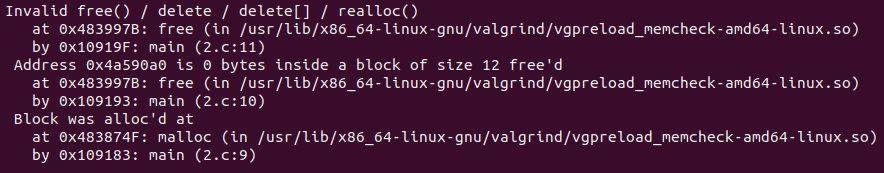
\includegraphics[width=0.9\textwidth]{InvalidFreeErrorPartOfResume.png}
%  \caption{Ispis greške nevalidnog oslobađanja memorije}
%  \label{fig:slika4.9}
%\end{figure} 

\begin{lstlisting}[style=terminal,caption={Ispis greške nevalidnog oslobađanja memorije}, label={lst:slika4.9},language={bash}]   
==2638==  Invalid free() / delete / delete[] / realloc()
==2638==      at 0x483997B: free (in /usr/lib/x86_64-linux-gnu/valgrind/vgpreload_memcheck-amd64-linux.so) 
==2638==      by Ox10919F: main (2.c:11)
==2638==  Address Ox4a590a0 is 0 bytes inside a block of size 12 free'd
==2638==      at 0x483997B: free (in /usr/lib/x86_64-linux-gnu/valgrind/vgpreload_memcheck-amd64-linux.so) 
==2638==      by 0x109193: main (2.c:10)
==2638==  Block was alloc'd at
==2638==      at Ox483874F: malloc (in /usr/lib/x86_64-linux-gnu/valgrind/vgpreload_memcheck-amd64-linux.so) 
==2638==      by 0x109183: main (2.c:9)
\end{lstlisting}

\subsection{Sumnjive vrednosti argumenata}
Šablon koji ispravlja greške sumnjivih vrednosti argumenata mapiran je na osnovu opisa koji daje alat \textit{Memcheck}, tj.~\textit{,,Argument 'size' of function x has a fishy (possibly negative) value: y''}, gde je \textit{x} naziv funkcije, a \textit{y} vrednost argumenta. Za ovaj tip greške mapiranje se vrši samo nad opisom greške, kako je sam razlog nedozvoljena vrednost argumenta, što \textit{Memcheck} ispisuje u okviru opisa greške. Na listingu \ref{lst:slika4.10} prikazan je ispis greške koji koristimo da bismo je ispravili. Analizom ispisa sa slike dobijamo preciznu informaciju o liniji koda, kao i o fajlu gde gde je pozvana funkcija koja sadrži sumnjivi arugment. U zavisnosti od funkcije, odgovarajućim transformacijama nad linijom koda u kojoj je poziv te funkcije, nalazimo mesto gde je sumnjivi arugment. Nažalost, nije uvek moguće automatsko ispravljanje grešaka ovog tipa na uniforman način. Nedozvoljena vrednost argumenata može biti na primer posledica pogrešno sračunatog izraza, što nije moguće ispraviti automatski. Ispravka koja je implemntirana obezbeđuje da program nema \textit{Runtime Error}, pa omogućava da se vrši debagovanje i lakše pronađu semantičke greške programa. Dakle, ovu grešku ispravljamo tako što izmenimo sumnjivi argument u pozivu funkcije u okviru problematične linije ispravnim, odnosno računamo apsolutnu vrednost sumnjivog argumenta. 

%\begin{figure}[!ht]
%  \centering
%  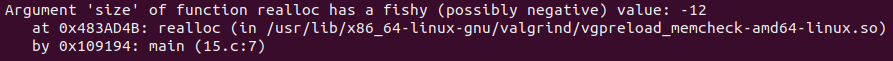
\includegraphics[width=0.9\textwidth]{reallocFishyArgument.png}
%  \caption{Ispis greške sumnjive vrednosti argumenta}
%  \label{fig:slika4.10}
%\end{figure} 

\begin{lstlisting}[style=terminal,caption={Ispis greške sumnjive vrednosti argumenta}, label={lst:slika4.10},language={bash}]   
==3565==  Argument 'size' of function realloc has a fishy (possibly negative) value: -12
==3565==      at Ox483AD4B: realloc (in /usr/lib/x86_64-linux-gnu/valgrind/vgpreload_memcheck-amd64-linux.so) 
==3565==      by 0x109194: main (15.c:7)
\end{lstlisting}

\subsection{Korišćenje neadresirane ili neinicijalizovane vrednosti u sistemskom pozivu}
Šablon koji ispravlja greške korišćenja neadresirane ili neinicijalizovane vrednosti u sistemskom pozivu mapiran je na osnovu opisa koji daje alat \textit{Memcheck}, npr.~\textit{,,Syscall param write(buf) points to uninitialised byte(s)''}, \textit{,,Syscall param exit\_group(status) contains uninitialised byte(s)''}, ili nekim drugim opisom karakterističnim za određenu vrstu funkcije. Za ovaj tip greške mapiranje se vrši samo nad opisom greške, kako grešku izazivaju loši argumenti funkcija sistemskog poziva. Na listingu \ref{lst:slika4.11} prikazan je jedan od ispisa ove greške, u konkretnom slučaju korišćenja funkcije \textit{write} koji koristimo da bismo je ispravili. Analizom ispisa sa slike dobijamo preciznu informaciju o liniji koda, kao i o fajlu gde gde je pozvana funkcija koja izaziva grešku, kao i linije koda gde je definisana neinicijalizovana ili neadresirana vrednost koja je u pozivu funkcije iskorišćena. Ispravka greške sastoji se u pronalaženju linije gde je definisana promenljiva i njena zamena ispravljenom linijom ili blokom koda koji sadrži tu liniju i dodatni k\^od koji ispravlja grešku.  

\begin{lstlisting}[style=terminal,caption={Primer ispisa greške korišćenja neinicializovane ili neadresirane vrednosti u sistemskom pozivu}, label={lst:slika4.11},language={bash}] 
==5695==  Syscall param write(buf) points to uninitialised byte(s)
==5695==     at 0x25A48723: __write_nocancel (in /lib/tls/libc-2.3.3.so)
==5695==     by 0x259AFAD3: __libc_start_main (in /lib/tls/libc-2.3.3.so)
==5695==     by 0x8048348: (within /auto/homes/njn25/grind/head4/a.out)
==5695==   Address 0x25AB8028 is 0 bytes inside a block of size 10 alloc'd
==5695==     at 0x259852B0: malloc (vg_replace_malloc.c:130)
==5695==     by 0x80483F1: main (a.c:5)
\end{lstlisting}

\section{Primeri rada alata}
U ovoj sekciji biće predstavljeni primeri rada alata za svaku od grešaka koje alat ispravlja. Prvi primer će dati kompletan pregled onoga što alat \textit{Koronka} radi sa programom koji analizira i šta ostavlja nakon svog rada. Ostali primeri biće izneti u formi listinga sa sledećom sadržinom:
\begin{itemize}
\item[$\textendash$] program koji sadrži greške;
\item[$\textendash$] ispravljeni program alatom \textit{Koronka};
\item[$\textendash$] izveštaj koji je formirao alat \textit{Koronka}.
\end{itemize} 

Primeri koji su prikazani u ovoj sekciji deo su skupa test primera koji se nalaze u direktorijumu \textit{Examples} u okviru glavnog direktorijuma alata. Podeljeni su po direktorijumima tako da svaki direktorijum sadrži program koji sadrži određene vrste grešaka. Takođe, mogu se naći i pokretanja i ispravke koje je \textit{Koronka} implementirala nad tim test primerima. Ti fajlovi smešteni su u odgovarajući direktorijum formata \textit{datum pokretanja-vreme pokretanja}, koje je alat \textit{Koronka} kreirala prilikom izvršavanja. Skup test primera dostupan je na linku \url{https://github.com/LMladenovic/Error_fixing_tool/tree/master/Examples}.  

Analiza i ispravka programa sa slike \ref{fig:slika4.15} predstavljena je u ovom primeru. 

\begin{figure}[!ht]
  \centering
  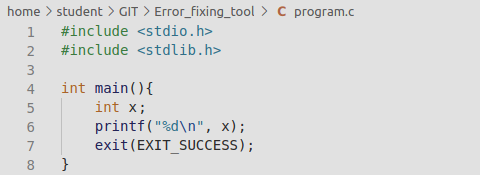
\includegraphics[width=0.6\textwidth]{ProgramWithError.png}
  \caption{Izgled programa koji sadrži grešku}
  \label{fig:slika4.15}
\end{figure}

Dati program sadrži grešku upotrebe neinicijalizovane promenljive koja će biti ispravljena. Alat pokrećemo komandom u komandnoj liniji:
\begin{center}
\textit{python koronka.py program.c}.
\end{center}

Izgled komandne linije nakon pokretanja alata prikazan je na slici \ref{fig:slika4.11}. 
\begin{figure}[!ht]
  \centering
  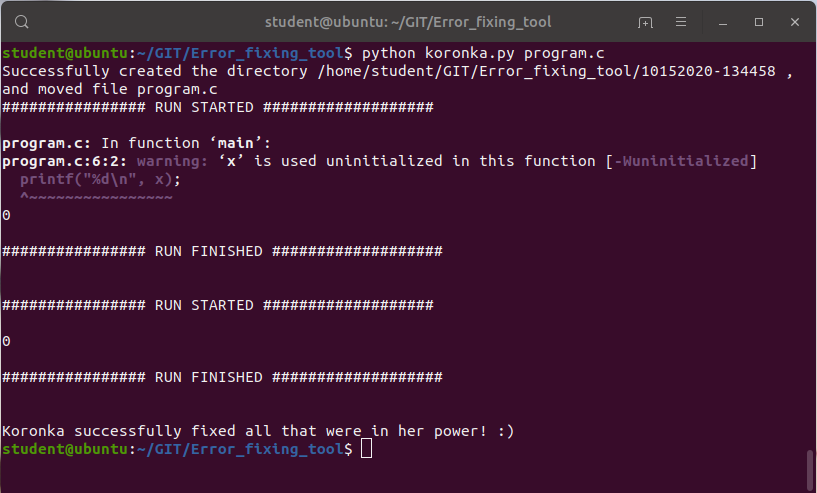
\includegraphics[width=0.6\textwidth]{TerminalOutput.png}
  \caption{Izgled terminala nakon izvršavanja alata \textit{Koronka}}
  \label{fig:slika4.11}
\end{figure}

Direktorijum koji je formiran i dodeljen ovom konkretnom pokretanju alata i njegovom izvršavanju prikazan je na slici \ref{fig:slika4.12}, dok su izmenjen program nakon izvršavanja alata \textit{Koronka}, kao i izveštaj, prikazani na slikama \ref{fig:slika4.13} i \ref{fig:slika4.14}.
\begin{figure}[!ht]
  \centering
  
\includegraphics[width=0.6\textwidth]{DateTimeFolder.png}
  \caption{Izgled foldera u formatu \textit{datum pokretanja - vreme pokretanja} koji formira alat \textit{Koronka}}
  \label{fig:slika4.12}
\end{figure}

\begin{figure}[!ht]
  \centering
  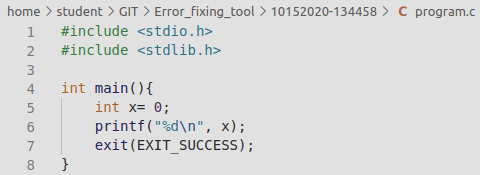
\includegraphics[width=0.6\textwidth]{FixedProgram.png}
  \caption{Izgled ispravljenog programa alatom \textit{Koronka}}
  \label{fig:slika4.13}
\end{figure}

\begin{figure}[!ht]
  \centering
  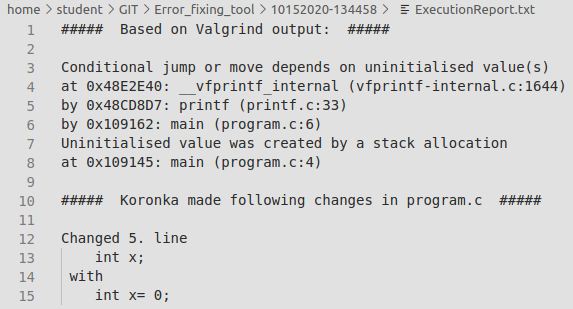
\includegraphics[width=0.6\textwidth]{ExecutionReport.png}
  \caption{Izgled izveštaja nakon izvršavanja alata \textit{Koronka}}
  \label{fig:slika4.14}
\end{figure}

\newpage
Primer programa koji sadrži greške korišćenja neinicializovanih ili neadresiranih vrednosti u sistemskom pozivu dat je na listingu \ref{lst:program1}, dok su ispravljeni program alatom \textit{Koronka} i prateći izveštaj dati na listinzima \ref{lst:program1Fix} i \ref{lst:program1Report}.

\begin{lstlisting}[style=mystyle,caption={Program koji sadrži greške korišćenja neinicializovanih ili neadresiranih vrednosti u sistemskom pozivu}, label={lst:program1},language={Python}] 
#include <stdlib.h>
#include <unistd.h>

int main( void ){
  char* arr  = malloc(10);
  int*  arr2 = malloc(sizeof(int));
  write( 1 /* stdout */, arr, 10 );
  exit(arr2[0]);
}
\end{lstlisting}

\begin{lstlisting}[style=mystyle,caption={Ispravljeni program sa listinga \ref{lst:program1} alatom \textit{Koronka}}, label={lst:program1Fix},language={Python}] 
#include <stdlib.h>
#include <unistd.h>

int main( void ){
  char* arr  = calloc( sizeof(char), 10);
  int*  arr2 = malloc(sizeof(int));
  write( 1 /* stdout */, arr, 10 );
  exit(0);
}
\end{lstlisting}

\begin{lstlisting}[style=terminal,caption={Izveštaj o radu alata \textit{Koronka} za program sa listinga \ref{lst:program1}}, label={lst:program1Report},language={bash}]   
#####  Based on Valgrind output:  #####

Syscall param write(buf) points to uninitialised byte(s)
at 0x4978024: write (write.c:26)
by 0x10918E: main (16.c:7)
Address 0x4a59040 is 0 bytes inside a block of size 10 alloc'd
at 0x483874F: malloc (in /usr/lib/x86_64-linux-gnu/valgrind/vgpreload_memcheck-amd64-linux.so)
by 0x109166: main (16.c:5)
Uninitialised value was created by a heap allocation
at 0x483874F: malloc (in /usr/lib/x86_64-linux-gnu/valgrind/vgpreload_memcheck-amd64-linux.so)
by 0x109166: main (16.c:5)

#####  Koronka made following changes in 16.c  #####

Changed 5. line 
  char* arr  = malloc(10);
 with 
  char* arr  = calloc( sizeof(char), 10);

#####  Based on Valgrind output:  #####

Syscall param exit_group(status) contains uninitialised byte(s)
at 0x494C926: _Exit (_exit.c:31)
by 0x48B23A9: __run_exit_handlers (exit.c:132)
by 0x48B23D9: exit (exit.c:139)
by 0x1091B0: main (16.c:8)
Uninitialised value was created by a heap allocation
at 0x483874F: malloc (in /usr/lib/x86_64-linux-gnu/valgrind/vgpreload_memcheck-amd64-linux.so)
by 0x109189: main (16.c:6)

#####  Koronka made following changes in 16.c  #####

Changed 8. line 
  exit(arr2[0]);
 with 
  exit(0);
\end{lstlisting}

Primer programa koji sadrži grešku nevalidnog oslobađanja memorije dat je na listingu \ref{lst:program2}, dok su ispravljeni program alatom \textit{Koronka} i prateći izveštaj dati na listinzima \ref{lst:program2Fix} i \ref{lst:program2Report}.

\begin{lstlisting}[style=mystyle,caption={Program koji sadrži grešku nevalidnog oslobađanja memorije}, label={lst:program2},language={Python}] 
#include <stdio.h>
#include <stdlib.h>

int main()
{
  char *p, q;

  p = (char *) malloc(19);
  p = (char *) malloc(12);
  free(p);
  free(p);

  p = &q;
  free(p); 			
  				
  return 0;
}
\end{lstlisting}

\begin{lstlisting}[style=mystyle,caption={Ispravljeni program sa listinga \ref{lst:program2} alatom \textit{Koronka}}, label={lst:program2Fix},language={Python}] 
#include <stdio.h>
#include <stdlib.h>

int main()
{
  char *p, q;

  p = (char *) malloc(19);
  p = (char *) malloc(12);
  free(p);


  p = &q;

  				
  return 0;
}
\end{lstlisting}

\begin{lstlisting}[style=terminal,caption={Izveštaj o radu alata \textit{Koronka} za program sa listinga \ref{lst:program2}}, label={lst:program2Report},language={bash}]   
#####  Based on Valgrind output:  #####

Invalid free() / delete / delete[] / realloc()
at 0x483997B: free (in /usr/lib/x86_64-linux-gnu/valgrind/vgpreload_memcheck-amd64-linux.so)
by 0x10919F: main (2.c:11)
Address 0x4a590a0 is 0 bytes inside a block of size 12 free'd
at 0x483997B: free (in /usr/lib/x86_64-linux-gnu/valgrind/vgpreload_memcheck-amd64-linux.so)
by 0x109193: main (2.c:10)
Block was alloc'd at
at 0x483874F: malloc (in /usr/lib/x86_64-linux-gnu/valgrind/vgpreload_memcheck-amd64-linux.so)
by 0x109183: main (2.c:9)

#####  Koronka made following changes in 2.c  #####

Removed 11. line
  free(p);

#####  Based on Valgrind output:  #####

Invalid free() / delete / delete[] / realloc()
at 0x483997B: free (in /usr/lib/x86_64-linux-gnu/valgrind/vgpreload_memcheck-amd64-linux.so)
by 0x1091A7: main (2.c:14)
Address 0x1ffefffcef is on thread 1's stack
in frame #1, created by main (2.c:5)

#####  Koronka made following changes in 2.c  #####

Removed 14. line
  free(p); 			
\end{lstlisting}

Primer programa koji sadrži grešku nevalidnog čitanja/pisanja dat je na listingu \ref{lst:program3}, dok su ispravljeni program alatom \textit{Koronka} i prateći izveštaj dati na listinzima \ref{lst:program3Fix} i \ref{lst:program3Report}.

\begin{lstlisting}[style=mystyle,caption={Program koji sadrži grešku nevalidnog čitanja/pisanja}, label={lst:program3},language={Python}] 
#include <stdio.h>
#include <stdlib.h>

int main(){

	int *t = malloc(4*sizeof(int));

	printf("Right side overdraft: %d\n", t[4]);
	printf("Left side overdraft: %d\n", t[4-5]);
	free(t); 
	return 0;
}
\end{lstlisting}

\begin{lstlisting}[style=mystyle,caption={Ispravljeni program sa listinga \ref{lst:program3} alatom \textit{Koronka}}, label={lst:program3Fix},language={Python}] 
#include <stdio.h>
#include <stdlib.h>

int main(){

	int *t = malloc(4*sizeof(int) + 1*sizeof(int));
		int __index__;
	for( __index__ = 0; __index__ < 5; __index__ ++)
		t[__index__] = 0;


	printf("Right side overdraft: %d\n", t[4]);
	printf("Left side overdraft: %d\n", t[abs(4-5)]);
	free(t); 
	return 0;
}
\end{lstlisting}

\begin{lstlisting}[style=terminal,caption={Izveštaj o radu alata \textit{Koronka} za program sa listinga \ref{lst:program3}}, label={lst:program3Report},language={bash}]   
#####  Based on Valgrind output:  #####

Invalid read of size 4
at 0x109173: main (14.c:8)
Address 0x4a59050 is 0 bytes after a block of size 16 alloc'd
at 0x483874F: malloc (in /usr/lib/x86_64-linux-gnu/valgrind/vgpreload_memcheck-amd64-linux.so)
by 0x109166: main (14.c:6)

#####  Koronka made following changes in 14.c  #####

Changed 6. line 
	int *t = malloc(4*sizeof(int));
 with 
	int *t = malloc(4*sizeof(int) + 1*sizeof(int));

#####  Based on Valgrind output:  #####

Conditional jump or move depends on uninitialised value(s)
at 0x48E2E40: __vfprintf_internal (vfprintf-internal.c:1644)
by 0x48CD8D7: printf (printf.c:33)
by 0x109187: main (14.c:8)
Uninitialised value was created by a heap allocation
at 0x483874F: malloc (in /usr/lib/x86_64-linux-gnu/valgrind/vgpreload_memcheck-amd64-linux.so)
by 0x109166: main (14.c:6)

#####  Koronka made following changes in 14.c  #####

Changed 6. line 
	int *t = malloc(4*sizeof(int) + 1*sizeof(int));
 with 
	int *t = malloc(4*sizeof(int) + 1*sizeof(int));
		int __index__;
	for( __index__ = 0; __index__ < 5; __index__ ++)
		t[__index__] = 0;

#####  Based on Valgrind output:  #####

Invalid read of size 4
at 0x1091BD: main (14.c:13)
Address 0x4a5903c is 4 bytes before a block of size 20 alloc'd
at 0x483874F: malloc (in /usr/lib/x86_64-linux-gnu/valgrind/vgpreload_memcheck-amd64-linux.so)
by 0x109166: main (14.c:6)

#####  Koronka made following changes in 14.c  #####

Changed 13. line 
	printf("Left side overdraft: %d\n", t[4-5]);
 with 
	printf("Left side overdraft: %d\n", t[abs(4-5)]);	
\end{lstlisting}

Primer programa koji sadrži grešku sumnjive vrednosti arguenata dat je na listingu \ref{lst:program4}, dok su ispravljeni program alatom \textit{Koronka} i prateći izveštaj dati na listinzima \ref{lst:program4Fix} i \ref{lst:program4Report}.

\begin{lstlisting}[style=mystyle,caption={Program koji sadrži grešku sumnjive vrednosti arguenata}, label={lst:program4},language={Python}] 
#include <stdio.h>
#include <stdlib.h>

int main(int argv, char** argc){
	char *r = malloc(-15);
	int *t = malloc(3);
	t = (int *)realloc(t, -3*sizeof(int)); 
	free(r);
	free(t);
	return 0;
}
\end{lstlisting}

\begin{lstlisting}[style=mystyle,caption={Ispravljeni program sa listinga \ref{lst:program4} alatom \textit{Koronka}}, label={lst:program4Fix},language={Python}] 
#include <stdio.h>
#include <stdlib.h>

int main(int argv, char** argc){
	char *r = malloc(abs(-15));
	int *t = malloc(3);
	t = (int *)realloc(t,abs( -3*sizeof(int))); 
	free(r);
	free(t);
	return 0;
}
\end{lstlisting}

\begin{lstlisting}[style=terminal,caption={Izveštaj o radu alata \textit{Koronka} za program sa listinga \ref{lst:program4}}, label={lst:program4Report},language={bash}]   
#####  Based on Valgrind output:  #####

Argument 'size' of function malloc has a fishy (possibly negative) value: -15
at 0x483874F: malloc (in /usr/lib/x86_64-linux-gnu/valgrind/vgpreload_memcheck-amd64-linux.so)
by 0x10916F: main (15.c:5)

#####  Koronka made following changes in 15.c  #####

Changed 5. line 
	char *r = malloc(-15);
 with 
	char *r = malloc(abs(-15));

#####  Based on Valgrind output:  #####

Argument 'size' of function realloc has a fishy (possibly negative) value: -12
at 0x483AD4B: realloc (in /usr/lib/x86_64-linux-gnu/valgrind/vgpreload_memcheck-amd64-linux.so)
by 0x109192: main (15.c:7)

#####  Koronka made following changes in 15.c  #####

Changed 7. line 
	t = (int *)realloc(t, -3*sizeof(int)); 
 with 
	t = (int *)realloc(t,abs( -3*sizeof(int))); 

\end{lstlisting}

Primer programa koji sadrži grešku za čije ispravljanje se koriste funkcije inicijalizacije korisnički definisanih struktura dat je na listingu \ref{lst:program5}, dok su ispravljeni program alatom \textit{Koronka} i prateći izveštaj dati na listinzima \ref{lst:program5Fix} i \ref{lst:program5Report}.

\begin{lstlisting}[style=mystyle,caption={Program koji sadrži grešku za čije ispravljanje se koriste funkcije inicijalizacije korisnički definisanih struktura}, label={lst:program5},language={Python}] 
#include <stdio.h>
#include <stdlib.h>

typedef struct _point{
int x;
int y;
int consts[3];
}Point;

int main(){

	Point A;

	Point B[5];

	printf("Point A(%d,%d)\n", A.x, A.y);
	
	int i;
	for (i=0;i<5;i++)
		printf("B[%d] = (%d, %d)\n", i+1, B[i].x, B[i].y);

	return 0;
}
\end{lstlisting}

\begin{lstlisting}[style=mystyle,caption={Ispravljeni program sa listinga \ref{lst:program5} alatom \textit{Koronka}}, label={lst:program5Fix},language={Python}] 
#include <stdio.h>
#include <stdlib.h>

typedef struct _point{
int x;
int y;
int consts[3];
}Point;

int main(){

	Point A;
	A.x=0;
	A.y=0;
	int __index__;
	for( __index__ = 0; __index__ < 3; __index__ ++)
		A.consts[__index__] = 0;

	Point B[5];
	int __index2__;
	for( __index2__ = 0; __index2__ < 5; __index2__ ++){
			B[__index2__].x=0;
			B[__index2__].y=0;
			int __index3__;
			for( __index3__ = 0; __index3__ < 3; __index3__ ++)
				B[__index2__].consts[__index3__] = 0;
		
	}

	printf("Point A(%d,%d)\n", A.x, A.y);
	
	int i;
	for (i=0;i<5;i++)
		printf("B[%d] = (%d, %d)\n", i+1, B[i].x, B[i].y);

	return 0;
}
\end{lstlisting}

\begin{lstlisting}[style=terminal,caption={Izveštaj o radu alata \textit{Koronka} za program sa listinga \ref{lst:program5}}, label={lst:program5Report},language={bash}]   
#####  Based on Valgrind output:  #####

Conditional jump or move depends on uninitialised value(s)
at 0x48E2E40: __vfprintf_internal (vfprintf-internal.c:1644)
by 0x48CD8D7: printf (printf.c:33)
by 0x10917D: main (12.c:16)
Uninitialised value was created by a stack allocation
at 0x109149: main (12.c:10)

#####  Koronka made following changes in 12.c  #####

Changed 12. line 
	Point A;
 with 
	Point A;
	A.x=0;
	A.y=0;
	int __index__;
	for( __index__ = 0; __index__ < 3; __index__ ++)
		A.consts[__index__] = 0;

#####  Based on Valgrind output:  #####

Conditional jump or move depends on uninitialised value(s)
at 0x48E2E40: __vfprintf_internal (vfprintf-internal.c:1644)
by 0x48CD8D7: printf (printf.c:33)
by 0x109228: main (12.c:25)
Uninitialised value was created by a stack allocation
at 0x109145: main (12.c:10)

#####  Koronka made following changes in 12.c  #####

Changed 19. line 
	Point B[5];
 with 
	Point B[5];
	int __index2__;
	for( __index2__ = 0; __index2__ < 5; __index2__ ++){
		B[__index2__].x=0;
		B[__index2__].y=0;
		int __index3__;
		for( __index3__ = 0; __index3__ < 3; __index3__ ++)
			B[__index2__].consts[__index3__] = 0;
		
	}
\end{lstlisting}

% ------------------------------------------------------------------------------

% ------------------------------------------------------------------------------
\chapter{Zaključak}
Alatima \textit{Valgrind} distribucije mogu se otkriti greške i kritične tačke programa čijim ispravljanjem direktno poboljšavamo konzistentnost, funkcionalnost i performanse programa koji se razvija. Ručno otkrivanje tih grešaka obično je mukotrpan i najčešće neefikasan postupak. Srećom, alat \textit{Valgrind} je tu da pomogne u prevazilaženju tog problema. Alat \textit{Memcheck}, koji je deo \textit{Valgrind} distribucije, otkriva greške u radu sa memorijom koje mogu da dovedu do pada programa, a koje kompilator nije u mogućnosti da otkrije. Ostali alati \textit{Valgrind} distribucije mogu da otkriju druge probleme, poput grešaka u radu sa nitima i sl., čijom se detekcijom i ispravljanjem može doprineti performansama i boljem radu softvera koji se razvija. 

Nakon što analizom programa nekim od alata distibucije \textit{Valgrind} detektujemo greške, ukoliko postoje, neophodno je da razumemo izlaz koji nam je alat dao, i da na osnovu njega pokušamo da popravimo greške. Alat koji je razvijen u ovom radu pokušava da taj proces automatizuje, odnosno da razume izlaz koji je alat \textit{Memcheck} dao, i da na osnovu njega korišćenjem adekvatnih šablona ispravi otkrivene greške. Alat pokriva širok dijapazon grešaka, što ne isključuje da postoje greške koje mogu biti otkrivene daljim razvojem, a koje alat \textit{Koronka} u ovom trenutku ne pokriva. Greške koje alat \textit{Koronka} uspešno otklanja su :
\begin{itemize}
\item korišćenje neinicijalizovanih vrednosti kako primitivnog tipa, tako i korisnički definisanih struktura, bilo da su one statički definisane, ili dinamički alocirane;
\item nedozvoljeno čitanje i pisanje u memoriju, kako s leve, tako i s desne strane, a koja je dinamički alocirana;
\item sumnjive vrednosti argumenata;
\item nevalidna oslobađanja memorije;
\item nevalidni arugmenti sistemskih poziva.
\end{itemize}
Greške koje alat \textit{Koronka} nije u stanju da ispravi, a koje \textit{Memcheck} detektuje su specijalni slučajevi grešaka koje alat ispravlja, a koje šabloni ne pokrivaju, ili greške za koje šablon još uvek nije implementiran.
To su na primer greške nedozvoljenog čitanja i pisanja iz statičke memorije i greške prilikom korišćenja funkcija poput \textit{mmap} i \textit{memcpy}.

Što se daljeg razvoja alata tiče, mogu se kreirati novi i dodatno specijalizovati i unaprediti postojeći mehanizmi i šabloni. Kako struktura alata liči na mikro servis, alat se može iskoristiti kao deo nekog novog alata, ili kao odvojeni deo skupa alata. Takođe, može biti proširen dijapazon grešaka koji alat ispravlja korišćenjem ostalih alata distribucije \textit{Valgrind}. Na primer, može se iskoristiti alat \textit{Helgrind} koji detektuje greške u radu sa nitima. Nakon ispravljanja grešaka koje detektuje \textit{Memcheck}, program bi se prepustio na dalju iterativnu analizu alatu \textit{Helgrind}, i šablonima za ispravljanje grešaka u radu sa nitima, što je slično principu koji je već iskorišćen. Nažalost, alate poput \textit{Cachegrind}-a i \textit{Callgrind}-a nije moguće iskoristiti u ovakvoj arhitekturi, kako nije moguće iskoristiti automatsku analizu njihovih izveštaja za isprvljanje propusta na koje oni ukazuju.

% ------------------------------------------------------------------------------

% ------------------------------------------------------------------------------
% Literatura
% ------------------------------------------------------------------------------
\literatura

% ==============================================================================
% Završni deo teze i prilozi
\backmatter
% ==============================================================================

% ------------------------------------------------------------------------------
% Biografija kandidata
\begin{biografija}
  \textbf{Lazar Mladenović} rođen je 24.02.1996. u Leskovcu. Osnovnu školu završio je 2010. u Leskovcu, kao đak generacije i nosilac Vukove diplome. U tom periodu biva zainteresovan za programiranje, pa se može reći da mu je to odredilo dalji tok obrazovanja. Prirodno-matematički smer leskovačke Gimnazije završava 2014., takođe kao nosilac Vukove diplome.
  
  2014. upisuje Matematički fakultet u Beogradu, smer Primenjena matematika, da bi se  dve godine kasnije prebacio na smer Računarstvo i informatika. Isti završava 2019. godine. Nakon diplomiranja upisuje master studije na istom smeru i fakultetu. 
  
  Oblasti interesovanja uključuju pre svega razvoj i verifikaciju softvera, kao i primenu programiranja u auto industriji.  
    
\end{biografija}
% ------------------------------------------------------------------------------

\end{document}
